% !TeX root = ../algebra_lineal.tex

\documentclass[../algebra_lineal.tex]{subfiles}

\begin{document}

\section{Notación}

¿Explicar aquí notación del tal que (aunque estoy poniendo tal que todo el rato con palabras)? ¿Explicar aquí la notación del subset (aunque estoy intentando utilizar todo el rato subseteq)? ¿Explicar aquí que los superíndices no son potencias? ¿Introducción a la importancia del álgebra lineal? ¿Tal vez introducción a las estructuras algebraicas?

\section{Cuerpos}

Para formalizar el concepto de espacio vectorial, deberemos antes formalizar el conjunto de escalares, es decir, un conjunto ``de dimensión uno'', signifique lo que signifique eso, que podremos utilizar para multiplicar (``escalar'') vectores. Habitualmente usaremos $\R$ o $\Complex$, pero en esta sección vamos a intentar extraer las propiedades relevantes de estos dos conjuntos para definir una estructura algebraica abstracta, el \textit{cuerpo}, del que únicamente conoceremos sus propiedades.

Informalmente, las propiedades más relevantes son la existencia de las operaciones suma y multiplicación, que estas sean algebraicamente cerradas
(es decir, que al sumar o multiplicar dos elementos del cuerpo obtengamos otro elemento del cuerpo), que cumplan las propiedades asociativa, conmutativa
\footnote{En ocasiones se distinguen a los cuerpos que cumplen la propiedad conmutativa como \textit{cuerpos abelianos}, en este texto todos los cuerpos
 serán conmutativos} y distributiva, que existan elementos neutros (0 para la suma y 1 para la multiplicación), que exista el concepto de \textit{división} (es decir, que cada elemento tenga un inverso multiplicativo), el concepto de \textit{resta} (es decir, que cada elemento tenga un opuesto aditivo). Estas aplicaciones suma y resta no tienen por qué ser la suma y resta habituales que conocemos en $\R$ o $\Complex$, puede ser cualquier otra función que satisfaga las propiedades (en algunas situaciones ni siquiera tendría sentido la suma o multiplicación usual).

Analicemos ahora la definición formal.

\begin{definition}[Cuerpo]
    Decimos que $\K$ es un cuerpo si existen dos aplicaciones $+:\K \times \K \to \K$, $\cdot:\K \times \K \to \K$ llamadas respectivamente suma y multiplicación que satisfacen las siguientes propiedades:
    \begin{enumerate}
        \item Asociatividad de la suma y multiplicación: $a+(b+c)=(a+b)+c$, $a\cdot(b\cdot c)=(a\cdot b)\cdot c$
        \item Conmutatividad de la suma y multiplicación: $a+b=b+a$, $a\cdot b = b \cdot a$
        \item Distributividad de la multiplicación sobre la suma: $a \cdot (b+c) = (a \cdot b) + (a \cdot c)$
        \item Elemento neutro para la suma: $\exists 0 \in \K \st \forall a \in \K, \spc a+0=a$
        \item Elemento identidad para la multiplicación:  $\exists 1 \in \K \st \forall a \in \K, \spc a\cdot 1=a$
        \item \label{cuerpo_opuesto} Opuesto aditivo: $\forall a \in \K, \spc \exists {(-a)} \in \K \st a + (-a) = 0 $.
        \item \label{cuerpo_inverso} Inverso multiplicativo: $\forall a \neq 0 \in \K, \spc \exists {(a^{-1})} \in \K \st a \cdot (a^{-1}) = 1$
    \end{enumerate}    
\end{definition}

\begin{notation}
    En las propiedades \ref{cuerpo_opuesto} y \ref{cuerpo_inverso} de los opuestos e inversos, hemos realizado un pequeño abuso de notación por motivos de claridad. Lo que realmente indica la propiedad es que para cualquier $a \in \K$ existe otro elemento $b_a \in \K$ (indicamos con el subíndice que depende de $a$) tal que $a + b_a = 0$. Denotamos al elemento $b_a$ como $-a$. Análogamente hacemos lo propio con el inverso multiplicativo. 
\end{notation}

\begin{remark}
    Sea cual sea el cuerpo, contiene a todos los números naturales ya que si $n \in \N \implies n = 1 + 1 + \dots + 1 \in \K$ porque cada uno de los $1$ pertenece a $\K$, por lo que la suma pertenece también.
\end{remark}

Con esta definición de cuerpo hemos ampliado significativamente el rango de conjuntos que podemos usar. Sin embargo, surgen algunos casos patológicos, como por ejemplo $\Z_2 = \set{0, 1}$, el cuerpo de los enteros módulo 2 (es decir, se ejecuta la aritmética usualmente y finalmente colapsamos los pares al 0 y los impares al 1). Se deja como ejercicio al lector demostrar que efectivamente $\Z_2$ es un cuerpo (de hecho, $\Z_p$ es un cuerpo para todo $p$ primo, algo fuera del alcance de este texto). La patología de $\Z_2$ radica en que $1+1=0$. A menudo querremos dividir entre 2 en variadas demostraciones, por lo que impondremos un requisito especial a los cuerpos que utilizaremos. Para ello, debemos introducir la definición de \textit{característica}.

\begin{definition}
    Llamamos característica de $\K$ al mínimo número de veces que es necesario sumar el elemento identidad 1 en una suma para obtener el elemento neutro 0. Es decir, la característica es el entero positivo $n$ más pequeño tal que:
    \[
        \underbrace{1+\dots+1}_{n\, \, \mathrm{sumandos}} = 0
    \]  
\end{definition}

A partir de ahora, salvo que mencionemos expresamente lo contrario, siempre hablaremos de cuerpos $\K$ de característica distinta de 2 (es decir, $1+1 \ne 0$).

\section{Espacios vectoriales}

Al igual que hicimos con los cuerpos, vamos a definir los espacios vectoriales usando únicamente las propiedades que lo definen. Más adelante relacionaremos esta definición con el concepto intuitivo de espacio vectorial utilizando coordenadas.

Al contrario que hicimos con los cuerpos, para definir un espacio vectorial necesitaremos un cuerpo $\K$ de característica distinta de 2, que utilizaremos para multiplicar los vectores, por lo que el cuerpo aparecerá en la definición de espacio vectorial.

\begin{definition}[Espacio vectorial]
    \label{vector_space_definition}
    Un conjunto $V \neq \emptyset$ es un espacio vectorial sobre $\K$ (también diremos que es un $\K$-espacio vectorial) si existen las siguientes operaciones en $V$ (suma y multiplicación por escalar) 
    
    \begin{multicols}{2}
        \noindent
        \begin{align*} +: V \times V &\to V \\
                (\vx, \vy) &\mapsto \vx + \vy
        \end{align*}
        \begin{align*}
            \cdot: \K \times V &\to V \\
                (a, \vx) &\mapsto a \vx
        \end{align*}
    \end{multicols}

    y satisfacen las siguientes propiedades:

    \begin{enumerate}
        \item Conmutatividad de la suma: $\forall \vx, \vy \in V, \spc \vx + \vy = \vy + \vx$
        \item Asociatividad de la suma: $\forall \vx, \vy, \vz \in V, \spc \vx + (\vy + \vz) = (\vx + \vy) + \vz$
        \item \label{espacio_vectorial_neutro} Elemento neutro: $\exists \zv \in V \st \forall \vx \in V, \spc \vx + \zv = \vx$
        \item \label{espacio_vectorial_opuesto} Elemento opuesto: $\forall \vx \in V, \spc \exists {({-x})} \in V \st  \vx + (-\vx) = \zv$
        \item Distributiva vectorial: $\forall a \in \K, \spc \forall \vx, \vy \in V, \spc a(\vx + \vy) = a\vx + a \vy$
        \item Distributiva escalar: $\forall a, b\in \K, \spc \forall \vx \in V, \spc (a+b)\vx = a\vx + b\vx$ 
        \item Asociativa: $\forall a, b \in \K, \spc \forall \vx \in V, \spc a \cdot (b \cdot \vx) = (a\cdot b) \cdot \vx $
        \item \label{espacio_vectorial_unidad} Elemento unidad: $\forall \vx \in V, \spc 1 \cdot \vx = \vx$ 
    \end{enumerate}

\end{definition}

\begin{remark}
    Es importante distinguir el elemento neutro $0 \in \K$ del cuerpo escalar, del elemento neutro $\zv \in V$ del espacio vectorial, ya que uno es un vector y otro un escalar. Sin embargo, el elemento identidad $1 \in \K$ de la propiedad \ref{espacio_vectorial_unidad} sí que es un escalar (se suman vectores, y se multiplican vectores con escalares).  
\end{remark}

\begin{notation}
    Si $V$ es un \kvspace, llamaremos a los elementos de V \textit{vectores} y a los elementos de $\K$ escalares.
\end{notation}

\begin{notation}
    A veces, para remarcar las operaciones de suma y multiplicación por escalar, diremos que $\parens{V, +, \cdot}$ es un \kvspace, pero usualmente omitiremos las operaciones, que se darán por sobreentendidas.
\end{notation}

A partir de ahora, si no indicamos otra cosa, $V$ será un \kvspace, siendo $\K$ un cuerpo de característica distinta de 2.

Es posible que esta definición abstracta de espacio vectorial parezca al lector algo árida, sin embargo es una herramienta muy potente que nos permitirá desarrollar una teoría que se puede aplicar a cualquier conjunto que satisfaga la definición de espacio vectorial, no únicamente a $\K^n$. Ejemplos de espacios vectoriales muy útiles en las matemáticas son los polinomios $\K[x]$ \footnote{Denotaremos como $\K[x]$ el conjunto de polinomios de cualquier grado sobre la variable $x$, es decir, polinomios de la forma, $a_n x^n + \dots + a_1 x + a_0$ con $a_i \in \K \spc \forall i \in {1, \dots, n}$}, las funciones continuas, las soluciones de ecuaciones diferenciales lineales, etc. Si desarrollamos todo desde las propiedades de espacio vectorial, podremos aplicar toda la teoría que desarrollemos a todos esos espacios vectoriales y muchos otros, sin tener que distinguir casos durante el desarrollo de la teoría.

A pesar de la potencia de esta aproximación a la definición de espacio vectorial, debemos demostrar incluso las cosas más nimias desde las propiedades. Comenzamos demostrando algunas propiedades inmediatas.

\begin{proposition}
    Sea $V$ un \kvspace. Entonces, las siguientes propiedades son ciertas:
    \begin{enumerate}
        \item $a \cdot \zv = \zv \spc \forall a \in \K$
        \item $a(-\vx) = -a\cdot \vx \spc \forall a \in \K$
        \item $0 \cdot \vx = \zv \spc \forall \vx \in V$
        \item \label{propiedad_cuatro_espacios_vectoriales} $(-a)\cdot \vx = -a\vx$
        \item Si $\vx \ne 0$, entonces $a \cdot \vx = \zv \implies a = 0$
    \end{enumerate}
\end{proposition}

\begin{proof}
    \begin{enumerate}[wide, labelwidth=0pt, labelindent=0pt]
        \item Primero observamos que $a\cdot \zv = a(\zv + \zv) = a \cdot \zv + a \cdot \zv $. Restando a ambos lados $a\cdot \zv$ obtenemos que 
            \[\zv = a\cdot \zv + (-a\cdot \zv) = (a \cdot \zv + a \cdot \zv) + (-a \cdot \zv) =  a \cdot \zv + \underbrace{(a \cdot \zv + (-a \cdot \zv))}_{\zv} = a \cdot \zv \]
        \item Primero nos percatamos de que $\zv = a \cdot \zv = a(\vx + (-\vx)) = a\vx +a\cdot(-\vx)$. Como $\zv$ es igual a dicha expresión, podemos sustituir la expresión de la derecha en cualquier lugar en el que aparezca $\zv$ por lo que
         \[ -a\vx = -a\vx + \zv = -a\vx + (a\vx + a(-\vx)) = \underbrace{(-a\vx + a\vx)}_{\zv} + a(-\vx) = a(-\vx) \] 
        \item En primer lugar vemos que $0 \cdot \vx = (0+0)\vx = 0 \cdot \vx + 0 \cdot \vx$. De nuevo, podremos sustituir eso en la siguiente ecuación
        \[\zv  = 0 \cdot \vx +(-0\cdot \vx) = (0\cdot \vx + 0\cdot \vx) + (-0\cdot \vx) =  0\cdot \vx + \underbrace{(0\cdot \vx + (-0\cdot \vx))}_{\zv} = 0\cdot\vx\]
        \item Observamos que $\zv = 0 \cdot \vx = (a + (-a))\vx = a\vx + (-a)\vx$. Sumar $\zv$ es equivalente a no hacer nada, por lo que podremos sumar la expresión de la derecha sin cambiar ningún vector
        \[-a\vx = -a\vx + (a\vx + (-a)\vx) = \underbrace{(-a\vx + a\vx)}_{\zv} + (-a)\vx = (-a)\vx \]
        \item Lo demostraremos por reducción al absurdo. Supongamos que $a \neq 0$, entonces $\frac{1}{a} \in \K$. Por tanto
        \[\vx = \underbrace{\left(\frac{a}{a} \right)}_{1} \vx = \frac{1}{a} (a \cdot \vx) = \frac{1}{a} \cdot \zv = \zv\]
        Hemos llegado a que $\vx = 0$, lo que es una contradicción.
    \end{enumerate}
\end{proof}

\begin{notation}
    Utilizaremos la notación usual en la que restar significa sumar el opuesto, es decir, $\vx - \vy = \vx + (-\vy)$
\end{notation}

\begin{remark}
    Si particularizamos la propiedad \ref{propiedad_cuatro_espacios_vectoriales} para $a=1$, obtenemos que $-\vx = (-1)\vx$, por lo que para obtener el vector opuesto basta con multiplicar por el opuesto del escalar $1$ (es decir, por $-1$).
\end{remark}

\begin{example}
    Veamos varios ejemplos de espacios vectoriales:
    \begin{itemize}
        \item Un cuerpo es un espacio vectorial sobre él mismo: $\K$ es un \kvspace.
        \item $\R$ es un $\Q$-espacio vectorial definiendo la suma y el producto usualmente
        
        \begin{multicols}{2}            
            \noindent\begin{align*}
                +: \R \times \R &\to \R \\
                    (a, b) &\mapsto a+b
            \end{align*}
            \begin{align*}
                \cdot: \Q \times \R &\to \R \\
                    \parens{\frac{p}{q}, a} &\mapsto \frac{p \cdot a}{q}
            \end{align*}
        \end{multicols}

        \item Si $n \in \N$, $\K^n$ es un espacio vectorial definiendo la suma de tuplas como la suma elemento a elemento y la multiplicación de una tupla por un escalar como la multiplicación de cada elemento de la tupla por dicho escalar, es decir,
        \begin{align*} +: \K^n \times \K^n &\to \K^n \\
                \parens{\parens{\dlst{a}{n}}, \parens{\dlst{b}{n}}} &\mapsto \parens{a_1+b_1, a_2+b_2, \dots, a_n+b_n}
        \end{align*}
        \begin{align*}
            \cdot: \K \times \K^n &\to \K^n \\
                (\lambda, \parens{\dlst{a}{n}}) &\mapsto \parens{\lambda \cdot a_1, \lambda \cdot a_2, \dots, \lambda \cdot  a_n}
        \end{align*}

    \end{itemize}
\end{example}

\section{Subespacios vectoriales}

En matemáticas es muy común querer trabajar con subconjuntos de un conjunto más grande. Habrá ocasiones en las que nos convenga trabajar por ejemplo con rectas o planos en vez de con el espacio vectorial total. Sin embargo, queremos que esos subconjuntos sigan teniendo la estructura de espacio vectorial, para poder aplicar a ellos también toda la teoría que estamos desarrollando. Nace de ahí el concepto de \textit{subespacio vectorial}, que informalmente es un subconjunto que con las \textbf{operaciones inducidas} del espacio vectorial que le contiene, sigue siendo a su vez un espacio vectorial. Es muy importante que las operaciones sigan siendo las mismas, es decir, la suma es la misma que en el espacio vectorial \textit{ambiente} (el espacio vectorial que lo contiene), para después poder juntar y usar varios subespacios vectoriales a la vez.

Para que las operaciones inducidas puedan ser efectivamente las operaciones de un espacio vectorial, estas deben ser cerradas. Es decir, la suma de vectores en el subespacio vectorial debe de seguir estando en el subespacio vectorial, y la multiplicación de un vector del subespacio por un escalar debe seguir estando en el subespacio. Esto es una condición necesaria para que un subconjunto sea subespacio vectorial, y es tan importante que hasta merece nombre.

\begin{definition}
    Un subconjunto no vacío $L\subseteq V$ es parte estable si verifica:
    \begin{enumerate}
        \item $\forall \vx, \vy \in L \implies \vx + \vy \in L$
        \item $\forall \vx \in L, \spc \forall a \in \K \implies a\cdot \vx \in L$
    \end{enumerate}
\end{definition}

Estamos ahora en condiciones de definir qué es un subespacio vectorial (sabiendo que ser parte estable es condición necesaria).

\begin{definition}[Subespacio vectorial]
    Una parte estable $L$ de $V$ es un subespacio vectorial de $V$ si $L$ con las operaciones inducidas por las de $V$ en $l$ es un \kvspace.
\end{definition}

\begin{remark}
    Las operaciones inducidas por $V$ en $L$ están bien definidas únicamente si $L$ es parte estable, y son las siguientes:
    \begin{multicols}{2}
        \noindent
        \begin{align*} +: L \times L &\to L \\
                (\vx, \vy) &\mapsto \vx + \vy \in L
        \end{align*}
        \noindent
        \begin{align*}
            \cdot: \K \times L &\to L \\
                (a, \vx) &\mapsto a \vx \in L
        \end{align*}
    \end{multicols} 
\end{remark}

De hecho, ser parte estable no es solamente condición necesaria, sino que también es condición suficiente.

\begin{proposition}
    $L$ es parte estable si y solamente si $L$ es un subespacio vectorial
\end{proposition}

\begin{proof}
    Solamente debemos demostrar la suficiencia. Sea $L \subseteq V$ parte estable. Únicamente debemos demostrar las propiedades \ref{espacio_vectorial_neutro} y \ref{espacio_vectorial_opuesto} de la definición \ref{vector_space_definition} de espacio vectorial para ver que $L$ es un \kvspace, ya que el resto de propiedades se cumplen en $V$, por lo que particularmente se cumplen en $L$.
    
    \begin{enumerate}
        \setcounter{enumi}{3}
        \item Sea $\vx \in L$, entonces $-\vx = \underbrace{(-1)}_{\in \K} \cdot \underbrace{\vx}_{\in V} \in L$. Pertenece a $L$ por ser $L$ parte estable.
        \setcounter{enumi}{2}
        \item Sea $\vx \in L$, entonces $\underbrace{\vx}_{\in L} + \underbrace{(-\vx)}_{\in L} = \zv \in L$. De nuevo pertenece a $L$ por ser $L$ parte estable.
    \end{enumerate}
\end{proof}

\begin{remark}
    Si $L$ es un subespacio vectorial, entonces $\zv \in L$ por ser $L$ a su vez un espacio vectorial. Es decir, el vector $\zv$ pertenece a todos los subespacios de un espacio vectorial dado. Esto se traduce en que todas las rectas, planos, etc. pasan por el origen. A un lector acostumbrado a los espacios afines (que estudiaremos más adelante, donde si existen rectas que no pasen por el origen) le podría chocar esto.
\end{remark}

Las operaciones de las que disponen los espacios son la suma de vectores y multiplicación por escalares, que usualmente combinaremos para dar lugar a las \textit{combinaciones lineales}

\begin{definition}[Combinación lineal]
    \label{definicion_combinacion_lineal}
    Sean $p \in \N, \spc \dlst{\vx}{p} \in V, \spc \ulst{a}{p} \in \K$. Si $\vx = \lincomb{a}{x}{p}$, diremos que $\vx$ es combinación linear de $\dlst{x}{p}$ con coeficientes $\ulst{a}{p}$.

\end{definition}

\begin{remark}
    En la definición \ref{definicion_combinacion_lineal} los superíndices no indican exponentes ni potencias, sino que se usan para distinguir distintos escalares. Como regla general, indexaremos los escalares por superíndices y los vectores con subíndices por motivos de claridad.
\end{remark}

Las combinaciones lineales son especialmente importantes porque juntan de manera concisa las sumas y multiplicaciones por escalares. Permiten usualmente expresar las propiedades que normalmente se deberían enunciar por separado en una sola propiedad, utilizando combinaciones lineales en vez de sumas y multiplicaciones. 

El primer ejemplo de esto es que los subespacios vectoriales son los conjuntos que continenen a las combinaciones lineales de sus vectores.


\begin{proposition}
    $\emptyset \ne L \subseteq V$ es subespacio vectorial $\iff \forall p \in N, \spc \forall \dlst{x}{p} \in L, \spc \forall \ulst{a}{p} \in \K, \spc \lincomb{a}{x}{p} \in L$.
\end{proposition}

\begin{proof}
    Veamos las dos implicaciones por separado.
    \begin{enumerate}
        \item[\protect\fbox{$\Rightarrow$}] Supongamos que $L$ es subespacio vectorial y sea $p \in \N$ \\
        Sean $\dlst{x}{p} \in L, \spc \ulst{a}{p} \in \K, \spc \lincomb{a}{x}{p} \in L$. Entonces, $a^1 \vx_1, a^2\vx_2, \dots, a^p\vx_p \in L$ por ser $L$ subespacio vectorial, y de nuevo, por ser $L$ subespacio vectorial se da que $\lincomb{a}{x}{p} \in L$. 
        \item[\protect\fbox{$\Leftarrow$}] Si $L$ contiene las combinaciones lineales, particularmente contiene cada suma y cada multiplicación por escalar, así que es parte estable y por tanto espacio vectorial.
    \end{enumerate} 
\end{proof}

\section{Bases de espacios vectoriales}

No todos los subconjuntos son espacios vectoriales, pero nos puede interesar encontrar un subespacio vectorial que contenga a determinado conjunto sin que este sea el total. Después de introducir las combinaciones lineales en la sección anterior, no es descabellada la idea de definir el conjunto de todas las combinaciones lineales de otro conjunto.

\begin{definition}
    Sea $\emptyset \neq H \subseteq V$ un subconjunto de $V$ que puede ser o no ser un espacio vectorial. Definimos $\lspan{H}$ como el conjunto de todas las combinaciones lineales de $H$, es decir,
    \[
        \lspan{H} = \set{\lincomb{a}{x}{p} : p \in \N, \spc \dlst{x}{p} \in L, \spc \ulst{a}{p} \in \K}
    \]
\end{definition}

En las siguientes proposiciones veremos que $\lspan{H}$ efectivamente contiene a $H$ y que efectivamente es un subespacio vectorial.

\begin{proposition}
    $H \subseteq \lspan{H}$
\end{proposition}

\begin{proof}
    Si $\vx \in H \implies \underbrace{1}_{\in \K} \cdot \underbrace{\vx}_{\in H} = \vx \in \lspan{H} \implies H \subseteq \lspan{H}$
    $ $.
\end{proof}

\begin{proposition}
    $\lspan{H}$ es un subespacio vectorial de $V$.
\end{proposition}

\begin{proof}
    Veamos que $\lspan{H}$ es parte estable.

    Sean $\vx, \vy \in \lspan{H} \Rightarrow \exists p, q \in \N, \spc \dlst{\vx}{p}, \dlst{\vy}{q} \in H, \, \, \ulst{a}{p}, \ulst{b}{q} \in \K $
    tal que 
    \begin{align*}
        \vx &= \lincomb{a}{x}{p} \\
        \vy &= \lincomb{b}{y}{q}
    \end{align*}

    Entonces podemos representar $\vx + \vy$ como
    
    \[
        \vx + \vy = a^1\underbrace{\vx_1}_{\in H}+a^2\underbrace{\vx_2}_{\in H}+\dots+a^p\underbrace{\vx_p}_{\in H} + b^1\underbrace{\vy_1}_{\in H}+b^2\underbrace{\vy_2}_{\in H}+\dots+b^p\underbrace{\vy_p}_{\in H}
    \]

    Por tanto $\vx + \vy$ es una combinación lineal de vectores de $H$, por lo que $\vx + \vy \in \lspan{H}$. Analizemos ahora el producto por escalar. Sea $a \in \K, \vx \in \lspan{H} \implies \exists p \in \N, \space \exists \dlst{\vx}{p} \in H$ y también $\exists \ulst{a}{p} \in \K \st \vx = \lincomb{a}{x}{p}$.  Multiplicamos a ambos lados por $a$:
    \[a\cdot \vx = a \left( \lincomb{a}{x}{p} \right) = \underbrace{(a \cdot a^1)}_{\in \K}\underbrace{\vx_1}_{\in H} + \underbrace{(a \cdot a^2)}_{\in \K}\underbrace{\vx_2}_{\in H} + \dots + \underbrace{(a \cdot a^p)}_{\in \K}\underbrace{\vx_p}_{\in H}\]

    Por tanto $a\vx$ es una combinación lineal finita de vectores de $H$, por lo que $a\vx \in \lspan{H}$.

    Concluimos por tanto que $\lspan{H}$ es un subespacio vectorial.
\end{proof}

De hecho, $\lspan{H}$ no es solamente un subespacio vectorial que contiene a $H$, sino que es el subespacio vectorial más pequeño que contiene a $H$. 

\begin{proposition}
    Si $L$ es un subespacio vectorial de $V$ tal que $H \subseteq L \implies \lspan{H} \subseteq L$, es decir, $\lspan{H}$ es el subespacio más pequeño de los subespacios vectoriales que contienen a $H$.¡
\end{proposition}

\begin{proof}
Sea $\vx \in \lspan{H} \Rightarrow \exists p \in \N, \spc \dlst{x}{p} \in H, \spc \ulst{a}{p} \in \K$ tal que 

\[ \vx = a^1 \underbrace{\vx_1}_{\in H \subseteq L} +  a^2\underbrace{\vx_2}_{\in H \subseteq L} + \dots +  a^p \underbrace{\vx_p}_{\in H \subseteq L} \]

Como cada $\vx_i \in H \subseteq L$, entonces cada $\vx_i \in L$, por lo que $x$ es combinación lineal de vectores de $L$ y por ser $L$ un espacio vectorial, $\vx \in L$. Como esto se da para cada $\vx \in \lspan{H}$, $\lspan{H} \subseteq L$.
\end{proof}

\subsection{Sistemas generadores y linealmente independientes}

Hasta ahora hemos utilizado $\lspan{H}$ para encontrar un subespacio vectorial conociendo $H$. Sin embargo, podemos utilizarlo a la inversa. Dado un espacio vectorial $V$, si conseguimos expresarlo como $V=\lspan{H}$ para algún $H$ pequeño (por ejemplo, finito), sabemos que podemos expresar todos los vectores de $V$ como combinaciones lineales de vectores de $H$, lo cuál simplifica muchas cuentas.

Introduzcamos algunas definiciones basadas en esta idea.

\begin{definition}[Subespacio generado]
    Diremos que $\lspan{H}$ es el subespacio vectorial generado por $H$.
\end{definition}

\begin{definition}[Sistema de generadores]
    Diremos que $H$ es un sistema de generadores de $V$ si $\lspan{H} = V$.
\end{definition}

\begin{definition}[Finitamente generado]
    Diremos que $V$ es finitamente generado o de dimensión finita si existe un sistema de generadores de $V$ formado por un número finitio de elementos, es decir, si
    \[
        \exists p \in N, \spc \exists \dlst{x}{p} \in V \st \lspan{\set{\vlst{x}{p}}} = V
    \]  
\end{definition}

Durante este texto vamos a tratar únicamente con espacios vectoriales finitamente generados, no trataremos espacios vectoriales de dimensión infinita.

Ya hemos comentado anteriormente que cuanto más \textit{pequeño} sea $H$, más convenientes resultarán los cálculos, ya que podremos descomponer cualquier vector en una combinación lineal de menores vectores. Si uno de los vectores de $H$ fuese combinación lineal de los otros vectores, entonces no aportaría nada a $\lspan{H}$, podríamos eliminarlo y $\lspan{H'}$ seguiría manteniendose igual, y habríamos conseguido eliminar un vector de $H$. 

De este concepto nace la siguiente definición:

\begin{definition}[Familia linealmente dependiente]
    Si $p \ge 2$ y $\vlst{x}{p} \in V$. Diremos que la familia $\set{\vlst{x}{p}}$ es linealmente dependiente si uno de ellos es combinación lineal de los otros. En el caso $p=1$, un único vector es linealmente dependiente solo si es el vector nulo, en caso contrario, es linealmente independiente. Alternativamente, la familia $\set{\vlst{x}{p}}$ es linealmente dependiente si
    \[\exists i \in \set{1, 2, \dots, p} \st \vx_i \in \lspan{\set{\vlst{x}{i-1}, \vx_{i+1}, \dots, \vx_p}}
    \]
\end{definition}

Muchas veces nos resultará más útil hablar de \textit{familias linealmente independientes}.

\begin{definition}[Familia linealmente independiente]
    La familia $\set{\vlst{x}{p}}$ es linealmente independiente si no es linealmente dependiente. Alternativamente, $\set{\vlst{x}{p}}$ es linealmente independiente si
    \[\forall i \in \set{1, 2, \dots, p}, \spc \vx_i \notin \lspan{\set{\vlst{x}{i-1}, \vx_{i+1}, \dots, \vx_p}}
    \]
\end{definition}

Existe otra caracterización muy importante de la dependencia lineal, que nos permitirá más adelante demostrar resultados importantes.

\begin{proposition}
   Sean $\set{\vlst{x}{p}} \in V$. Entonces  $\set{\vlst{x}{p}}$ son linealmente dependientes si y solo si $\exists \slst{a}{p} \in \K$ no todos nulos tal que $\lincomb{a}{x}{p} = \zv$

\end{proposition}

\begin{proof}

    Analicemos las dos implicaciones por separado.
    \begin{enumerate}
        \item[\protect\fbox{$\Rightarrow$}] Supongamos $\set{\vlst{x}{p}}$ linealmente dependientes, es decir 
        \[\exists i \in \set{1, 2, \dots, p} \st \vx_i \in \lspan{\set{\vlst{x}{i-1}, \vx_{i+1}, \dots, \vx_p}}\]
        Por tanto, $\exists \slst{a}{i-1}, a^{i+1}, a^p \in \K$ tales que 
        \[
            \vx_i = \lincomb{a}{x}{i-1}+a^{i+1}\vx_{i+1}+\dots+a^p \vx_p  
        \]
        Restando $\vx_i$ a ambos lados de la ecuación llegamos a que
        \[
            \vx_i - \vx_i = \zv  = \lincomb{a}{x}{i-1}+\underbrace{(-1)}_{\ne 0}\vx_i +a^{i+1}\vx_{i+1}+\dots+a^p \vx_p
        \]
        \item[\protect\fbox{$\Leftarrow$}] Supongamos que $\exists \slst{a}{p} \in \K$ no todos nulos tal que $\lincomb{a}{x}{p} = 0$. Sea $i\in \set{1, \dots, p} \st a^i \ne 0 \Rightarrow \frac{1}{a} \in \K$. Por tanto,
        \begin{align*}
            \zv &= \frac{1}{a^i} \cdot \zv = \frac{1}{a^i}\parens{ \lincomb{a}{x}{i-1} + a^i\vx_i + a^{i+1}\vx_{i+1} + \dots a^p\vx_p} \\
                &= \parens{\frac{a^1}{a^i}}\vx_1 + \parens{\frac{a^2}{a^i}}\vx_2 + \dots + \parens{\frac{a^{i-1}}{a^i}}\vx_{i-1} + \underbrace{\parens{\frac{a^{i}}{a^i}}}_{1}\vx_{i} + \parens{\frac{a^{i+1}}{a^i}}\vx_{i+1} + \dots + \parens{\frac{a^{p}}{a^i}}\vx_{p}
        \end{align*}
        El coeficiente de $\vx_{i-1}$ es $1$, así que basta pasar el resto de términos que le acompañan restando para despejar $\vx_{i-1}$, obteniendo 
        \[
           \vx_{i} = \underbrace{\parens{\frac{-a^1}{a^i}}}_{\in \K}\vx_1 + \underbrace{\parens{\frac{-a^2}{a^i}}}_{\in \K}\vx_2 + \dots + \underbrace{\parens{\frac{-a^{i-1}}{a^i}}}_{\in \K}\vx_{i-1} + \underbrace{\parens{\frac{-a^{i+1}}{a^i}}}_{\in \K}\vx_{i+1} + \dots + \underbrace{\parens{\frac{-a^{p}}{a^i}}}_{\in \K}\vx_{p}
        \]

        Por tanto, $\vx_i$ es combinación lineal del resto de vectores.
    \end{enumerate}
\end{proof}

Negando los dos lados del si y solo si en la proposición anterior, conseguimos el siguiente corolario.

\begin{corollary}
    \label{linear_independence_corollary}
    Sean $\set{\vlst{x}{p}} \subseteq V$. Entonces $\set{\vlst{x}{p}}$ son linealmente independientes $\iff$ si  $\slst{a}{p} \in \K \st \lincomb{a}{x}{p} = \zv$ entonces $a^i = 0 \spc \forall i \in  \set{1, \dots, p} $. 
\end{corollary}

Una propiedad muy importante de las familias linealmente independientes, es que cualquier vector que se pueda expresar como combinación lineal de ellas se hace de manera única, es decir, no existen dos combinaciones lineales distintas de elementos de la familia. La demostración se apoya en la caracterízación que acabamos de demostrar.

\begin{proposition}
    Sean $\set{\vlst{x}{p}} \subseteq V$. Entonces son equivalentes:
    \begin{enumerate}[a)]
        \item $\set{\vlst{x}{p}}$ son linealmente independientes.
        \item Cualquier vector de $\lspan{\set{\vlst{x}{p}}}$ se puede expresar como una única combinación lineal.  Es decir, $\forall \vx \in \lspan{\set{\vlst{x}{p}}}, \spc \exists! \, \slst{a}{p} \in \K$ tal que $\vx = \lincomb{a}{x}{p}$. 
    \end{enumerate}
\end{proposition}

\begin{proof}

    Analicemos las dos implicaciones por separado.
    \begin{enumerate}[itemindent=20pt]
        \item[\protect\fbox{a) $\Rightarrow$ b)}] Supongamos que $\set{\vlst{x}{p}}$ son l.i. (linealmente independientes). \\
        Sea $\vx \in \lspan{\set{\vlst{x}{p}}} \Rightarrow \exists \slst{a}{p} \in \K \st \vx = \lincomb{a}{x}{p}$. Sean $\slst{a}{p} \in \K \st \vx = \lincomb{a}{x}{p}$. Entonces, restando:
        \begin{align*}
            \zv &= \vx - \vx = \lincomb{a}{x}{p} - (\lincomb{b}{x}{p}) = \\
                &= \parens{a^1-b^1}\vx_1 + \parens{a^2-b^2}\vx_2 + \dots + \parens{a^p-b^p}\vx_p
        \end{align*}
        Como hemos supuestos que $\set{\vlst{x}{p}}$ son l.i., por el corolario \ref{linear_independence_corollary} todos los coeficientes son 0, es decir,
        \[
            \begin{array}[t].{l}\}
            a^1-b^1 = 0 \\
            a^2-b^2 = 0 \\ 
            \hspace{12.74mm}\vdots \\
            a^p-b^p = 0
            \end{array}
            \begin{array}[t]{@{}c@{}}\\{}\implies {}\\{}\end{array}
            \begin{array}[t].{l}\}
                a^1 = b^1 \\
                a^2 = b^2 \\ 
                \hspace{5.3mm}\vdots \\
            a^p = b^p
            \end{array}
        \]
    
        \item[\protect\fbox{b) $\Rightarrow$ a)}] Supongamos que si $\vx \in \lspan{\set{\vlst{x}{p}}}, \spc \exists ! \, \slst{a}{p} \in \K $ tal que 
        \(\vx = \lincomb{a}{x}{p}\). Demostremos que $\set{\vlst{x}{p}}$ son linealmente independientes utilizando la caracterización. Sean $\slst{b}{p}\in \K$ tal que $\lincomb{b}{x}{p} = \zv$. Además, por ser $0\cdot \vx = \zv \spc \forall x \in V$, tenemos que $0 \cdot \vx_1 + 0 \cdot \vx_2 + \dots + 0 \cdot \vx_p = \zv$. El vector nulo se puede expresar entonces como dos combinaciones lineales:

        \[
        \begin{cases}
            \lincomb{b}{x}{p} &= \zv \\
            0 \cdot \vx_1 + 0 \cdot \vx_2 + \dots + 0 \cdot \vx_p &= \zv
        \end{cases}
        \]
        Como solamente existe una única combinación lineal que represente a $\zv$, entonces $b^i = 0 \spc \forall i \in \set{1, \dots, p} $ 
    \end{enumerate}
\end{proof}

    La siguiente proposición nos ayudará a expandir una familia de vectores que ya sabemos que son linealmente independientes con un nuevo vector bajo ciertas condiciones.

    \begin{proposition}
        Sean $\set{\vlst{x}{p}}$ linealmente independientes y sea $\vx \notin \lspan{\set{\vlst{x}{p}}}$, es decir, $\vx$ no es combinación lineal de $\set{\vlst{x}{p}}$. Entonces $\set{\vx, \vlst{x}{p}}$ son l.i.
    \end{proposition}

    \begin{proof}
        Sean $a,\slst{a}{p} \in \K$ tal que $a\vx + \lincomb{a}{x}{p} = 0$
        Veamos por reducción al absurdo que neecsariamente $a = 0$.
        \begin{enumerate}[itemindent=20pt]
            \item[\protect\fbox{si $a \ne 0$}] 
            \[
                \zv = \frac{1}{a} \cdot \zv = \frac{1}{a} \left( a\vx + a^1 \vx_1 + \dots + a^p\vx_p  \right) = \vx + \frac{a^1}{a}\vx_1 + \dots + \frac{a^p}{a}\vx_p
            \]
            Despejando $\vx$ restando
            \[
                \vx = \parens{\frac{-a^1}{a}}\vx_1 + \dots + \parens{\frac{-a^p}{a}}\vx_p
            \]
            Hemos llegado a una contradicción porque hemos podido expresar $\vx$ como combinación lineal de $\set{\vlst{x}{p}}$, por tanto, necesariamente $a=0$
            \item[\protect\fbox{si $a = 0$}] Como $a=0$, solamente necesitamos ver que $a_i=0 \spc \forall i \in \set{1, \dots, p}$.
            \[
                \zv = \underbrace{0 \cdot \vx}_{\zv} + \lincomb{a}{x}{p} = \lincomb{a}{x}{p}
            \] 

            Como $\set{\vlst{x}{p}}$ son l.i., $a_i=0 \spc \forall i \in \set{1, \dots, p}$. Como además $a=0$, tenemos que $\set{x, \vlst{x}{p}}$ son l.i.
        \end{enumerate}
    \end{proof}

    \begin{remark}
        A pesar de ser un error relativamente común, si existen 4 vectores linealmente independientes 3 a 3 entre sí, eso no implica que los 4 vectores sean linealmente independientes. Un contraejemplo de esto son los vectores $\set{(1,0,0),(0,1,0),(0,0,1),(1,1,1)}$ de $\R^3$.
    \end{remark}

\subsection{Teoremas de la base}

Hemos visto que si un conjunto de vectores es sistema generador, podemos expresar cualquier vector del espacio vectorial como una combinación lineal de elementos del conjunto. Además, si ese conjunto fuese linealmente independiente, podríamos expresar de manera única esa combinación lineal, lo cual es increíblemente útil.

\begin{definition}[Base]
    Una familia de vectores $\set{\vlst{u}{n}} \subseteq V$ es una base de $V$ si son un sistema de generadores de $V$ y son linealmente independientes.
\end{definition}

Como hemos dicho antes, cualquier vector se puede expresar de manera única como combinación lineal de vectores de la base. Más formalmente, si $\set{\vlst{u}{n}}$ es una base de $V$, Entonces
$$\forall \vx \in V, \spc \exists! \, \slst{a}{n} \in \K \st \vx = \lincomb{a}{u}{n}$$ 

\begin{remark}
    Una vez fijada una base, cada vector queda únicamente representado por los $n$ coeficientes únicos  $\slst{a}{n} \in \K$ de la combinación lineal. Podemos observar estos coeficientes como una tupla $\parens{\slst{a}{n}} \in \K^n$. Esto significa que independientemente de lo extraño que sea el espacio vectorial con el que estemos tratando, una vez fijada una base podemos trabajar con él \textit{como si fuera} $\K^n$. Formalmente esto se expresa creando una biyección $\phi$ desde $V$ hasta $\K^n$
    \begin{align*}
        \phi: V &\to \K^n \\
            \vx &\mapsto \parens{\slst{a}{n}}
    \end{align*} 
    siendo $\slst{a}{n}$ los únicos escalares tal que $\vx = \lincomb{a}{u}{n}$.
\end{remark}

Gracias a las buenas propiedades de las bases, sería muy afortunado que todo espacio vectorial finitamente generado tuviese una. Eso es precisamente lo que nos dice el primer teorema de la base.

\begin{theorem}[Primer teorema de la base]
    Sea $V \ne \set{\zv}$ finitamente generado, entonces $\exists \set{\vlst{u}{n}}$ base de $V$ 
\end{theorem}

\begin{proof}
    Si $V \ne \set{\zv}$ es finitamente generado, $\exists p \in \N, \spc \exists \vlst{x}{p} \in V$ tal que $\vlst{x}{p}$ es sistema de generadores de $V$. Pueden darse dos casos, si $\set{\vlst{x}{p}}$ son linealmente independientes, entonces son base y hemos demostrado lo que queríamos. En caso contrario, son linealmente dependientes, es decir
    \[
        \exists i \in \set{1, \dots, p} \st \vx_i \in \lspan{\set{\vlst{x}{i-1}, \vx_{i+1}, \dots, \vx_{p}}}
    \]
    Veamos que entonces $\set{\vx_{1}, \dots,  \vx_{i-1}, \vx_{i+1}, \dots, \vx_{p}}$ también es sistema de generadores de $V$. $\vx_i$ es por tanto combinación lineal del resto, por lo que $\exists \islst{a}{p}{i} \in \K$ tal que $\vx_i = \ilincomb{a}{x}{p}{i}$. Por ser $\set{\vlst{x}{p}}$ sistema de generadores, $\forall \vx \in V, \spc \exists \cslst{b}{p}{i} \in \K $ tal que 
    \begin{align*}
        \vx &= \clincomb{b}{x}{p}{i} \\
            &= b^1\vx_{1} + \dots + b^{i-1} \vx_{i-1} + b^i \parens{\ilincomb{a}{x}{p}{i}} + \\
            &\hspace{11.35mm} + b^{i+1} \vx_{i+1} + \dots + b^p \vx_p = \\
            &= \parens{b^1 + b^i a^1}\vx_{1} + \dots + \parens{b^{i-1} + b^i a^{i-1}}\vx_{i-1} + \parens{b^{i+1} + b^i a^{i-1}}\vx_{i+1} + \dots + \parens{b^p + b^i a^p}\vx_{p}
    \end{align*}
    Por tanto, podemos expresar cada $\vx$ como combinación lineal de $\set{\ivlst{x}{p}{i}}$, por lo que $\set{\ivlst{x}{p}{i}}$ es sistema de generadores de $V$. 
    Podemos repetir este método hasta que todos los vectores sean linealmente independientes. En el peor caso, aplicando este método $p-1$ veces, llegaremos a $\set{\vx_j}$. Como $V \ne \set{\zv}$, entonces $\vx_j \ne \zv \Rightarrow \set{\vx_j}$ es linealmente independiente.
\end{proof}

Demostraremos ahora un teorema, que a pesar de parecer tener un enunciado un tanto árido, nos permitirá deducir con facilidad que todas las bases de un espacio vectorial finitamente generado poseen el mismo número de vectores.

\begin{theorem}[Steinitz]
    Sea $\set{\vlst{x}{p}}$ un sistema de generadores de $V$ y consideremos $\set{\vlst{y}{q}}$ linealmente independientes. Entonces $q \le p$ y se puede obtener un nuevo sistema de generadores sustituyendo $q$ de los vectores $\vx_i$ por los $q$ vectores $\vlst{y}{q}$.
\end{theorem}

\begin{proof}
    Demostremos primero la segunda parte por inducción.
    \begin{enumerate}[itemindent=30pt]
        \item[\protect\fbox{Caso base}] $ $ \linebreak
    \end{enumerate}
    Como $\vy_1 \in V$ y $\set{\vlst{x}{p}}$ es sistema de generadores, entonces $\exists \slst{a}{p} \in \K$ tal que $\vy_1 = \lincomb{a}{x}{p}$. Como $\vy_1$ forma parte de una familia de vectores l.i., entonces $\parens{\slst{a}{p}} \ne \parens{0, 0, \dots, 0}$, es decir, no todas las $a^i$ son nulas. Sin pérdida de generalidad (podemos permutar los vectores $\vx_j$ para llevar el escalar no nulo hasta $a^1$), suponemos que $a^1\ne 0$. Por tanto,
    \begin{align*}
        \frac{1}{a^1}\vy_1 &= \frac{1}{a^1} \parens{\lincomb{a}{x}{p}} \\
                        &= \underbrace{\frac{a^1}{a^1}}_{1}\vx_1 + \frac{a^2}{a^1}\vx_2 + \dots + \frac{a^p}{a^1}\vx_p 
    \end{align*}
    Despejamos $\vx_1$ restando
    \[
        \vx_1 = \frac{1}{a^1}\vy_{1} + \frac{-a^2}{a^1}\vx_2 + \dots + \frac{-a^p}{a^1}\vx_p
    \]
    Veamos que $\set{\vy_1, \vx_2, \dots, \vx_p}$ es sistema de generadores de $V$. $\forall \vx \in V, \spc \exists \slst{\alpha}{p} \in \K$ tal que 
    \begin{align*}
        \vx &= \lincomb{\alpha}{x}{p} \\
            &= \alpha^1 \parens{\frac{1}{a^1}\vy_{1} + \frac{-a^2}{a^1}\vx_2 + \dots + \frac{-a^p}{a^1}\vx_p} + \alpha^2\vx_2 + \dots + \alpha^p\vx_p \\
            &= \frac{\alpha^1}{a^1}\vy_1 + \parens{\alpha^2 - \frac{a^2 \alpha^1}{a^1}}\vx_2 + \dots + \parens{\alpha^p - \frac{a^p \alpha^1}{a^1}}\vx_p
    \end{align*}
    Por tanto $\set{\vy_1, \vx_2, \dots, \vx_p}$ es sistema de generadores de $V$.
    \begin{enumerate}[itemindent=50pt]
        \item[\hspace{20mm}\protect\fbox{Paso inductivo}] $ $ \linebreak
    \end{enumerate}
    Supongamos que para $i < \min \braces{p, q}$ tenemos que $\set{\vy_1, \vy_2, \dots, \vy_{i}, \vx_{i+1}, \dots, \vx_p}$ es sistema de generadores de $V$. Como $\vy_{i+1} \in V, \spc \exists \slst{a}{i}, b^{i+1}, \dots, b^q \in \K$ tales que 
    \[
        \vy_{i+1} = \lincomb{a}{y}{i} + b^{i+1}\vx_{i+1} + \dots + b^p \vx_p 
    \]
    De nuevo, por formar $\vy_{i+1}$ parte de una familia l.i., $\parens{b^{i+1}, \dots, b^p} \ne \parens{0, \dots, 0}$. Sin pérdida de generalidad, supongamos que $b^{i+1} \ne 0$, por lo que
    \begin{align*}
        \frac{1}{b^{i+1}}\vy_{i+1} &= \frac{1}{b^{i+1}} \parens{\lincomb{a}{y}{i} + b^{i+1}\vx_{i+1} + \dots + b^p \vx_p} \\
                                   &= \frac{a^1}{b^{i+1}} \vy_1 + \frac{a^2}{b^{i+1}} \vy_2 + \dots + \frac{a^i}{b^{i+1}}\vy_i + \underbrace{\frac{b^{i+1}}{b^{i+1}}}_{1}\vx_{i+1} + \dots + \frac{b^{p}}{b^{i+1}}\vx_{p} 
    \end{align*}
    Despejando $\vx_{i+1}$
    \[
        \vx_{i+1} = \frac{-a^1}{b^{i+1}}\vy_1 + \frac{-a^2}{b^{i+1}}\vy_2 + \dots + \frac{-a^i}{b^{i+1}}\vy_i + \frac{1}{b^{i+1}} \vy_{i+1} + \frac{-b^{i+2}}{b^{i+1}}\vx_{i+2} +  \dots + \frac{-b^p}{b^{i+1}}\vx_p
    \]
    Vamos a demostrar que $\set{\vy_1, \vy_2, \dots, \vy_{i}, \vy_{i+1}, \dots, \vx_p}$ es sistema de generadores de $V$. Sea $\vx \in V, \spc \exists \slst{\alpha}{i},\beta^{i+1}, \dots, \beta^p \in \K$ tal que 
    \begin{align*}
        \vx &= \lincomb{\alpha}{y}{i} + \beta^{i+1}\vx_{i+1}+\dots  + \beta^p\vx_p \\
            &= \lincomb{\alpha}{y}{i} + \\
            &\hspace{5mm} + \beta^{i+1} \parens{\frac{-a^1}{b^{i+1}}\vy_1 + \frac{-a^2}{b^{i+1}}\vy_2 + \dots + \frac{-a^i}{b^{i+1}}\vy_i + \frac{1}{b^{i+1}} \vy_{i+1} + \frac{-b^{i+2}}{b^{i+1}}\vx_{i+2} +  \dots + \frac{-b^p}{b^{i+1}}\vx_p} + \\
            &\hspace{5mm} + \dots + \beta^p\vx_{p} \\
            &= \parens{\alpha^1 - \frac{\beta^{i+1}a^1}{b^{i+1}}} \vy_1 + \dots + \parens{\alpha^i - \frac{\beta^{i+1}a^i}{b^{i+1}}}\vy_i + \frac{\beta^{i+1}}{b^{i+1}}\vy_{i+1} + \dots + \parens{\beta^p - \frac{\beta^{i+1}b^p}{b^{i+1}}}\vx_p
    \end{align*}
    Por tanto, todos los vectores son combinación lineal de $\set{\vy_1, \vy_2, \dots, \vy_{i}, \vy_{i+1}, \dots, \vx_p}$, por lo que es sistema de generadores.
    \begin{enumerate}[itemindent=21pt]
        \item[\hspace{20mm}\protect\fbox{Si $p < q$}] $ $ \linebreak
    \end{enumerate}
    Demostramos por último la primera parte del teorema por reducción al absurdo. Supongamos que $p > q$. Sabemos que $\set{\vlst{y}{p}, \vy_{p+1}, \dots, \vy_{q}}$ son linealmente independientes. Como $\set{\vlst{x}{p}}$ es sistema de generadores, sustituyendo como antes, tenemos que $\set{\vlst{y}{p}}$ es sistema de generadores.  Sin embargo, por ser los $\vy_j$ linealmente independientes, $\vy_{i+1} \notin \lspan{\set{\vlst{y}{p}}}$. Hemos llegado a una contradicción, por lo que $p \ge q$.
\end{proof}

Estamos por fin en condiciones de demostrar que todas las bases tienen el mismo número de elementos.

\begin{corollary}[Segundo teorema de la base]
    Todas las bases de un espacio vectorial $V \ne {\zv}$ finitamente generado tienen el mismo número de elementos.
\end{corollary}

\begin{proof}
    Sean $\mathcal{B} = \set{\vlst{u}{n}}$ y $\mathcal{B'} = \set{\vlst{v}{m}}$ dos bases de $V$. Aplicamos dos veces el teorema de Steinitz:
    \begin{itemize}
        \item $\mathcal{B}$ es sistema de generadores y $\mathcal{B'}$ es una familia l.i. Aplicando Steinitz, $m \le n$
        \item $\mathcal{B'}$ es sistema de generadores y $\mathcal{B}$ es una familia l.i. Aplicando Steinitz, $n \le m$
    \end{itemize}

    Por tanto, como $n \le m$ y $m \le n$, tenemos que $m = n$
\end{proof}

Por tanto, el número de elementos de la base es algo inherente al espacio vectorial, y no a cada base, lo que motiva la siguiente definicion.

\begin{definition}[Dimensión]
    Llamaremos dimensión de $V \ne \set{\zv}$ al número de vectores de cualquier base de $V$. Lo notaremos como $\dim{V}$. Diremos que $\dim{\set{\zv}} = 0$.
\end{definition}

\begin{remark}
    Si $\dim{V} = n$ y $\set{\vlst{x}{p}} \subseteq V$ linealmente independientes, aplicando Steinitz tenemos que $p \le n$. Es decir, $\dim{V}$ es el número máximo de vectores que forman una familia linealmente independiente. Análogamente, si $\set{\vlst{x}{p}} \subseteq V$ sistema de geeradores, aplicando Steinitz tenemos que $n \le p$. Es decir, $\dim{V}$ es el mínimo número de vectores que forman un sistema de generadores de $V$. 
\end{remark}

\begin{example}
    La dimensión de un espacio puede cambiar dependiendo del cuerpo con el que se considere el espacio vectorial. Por ejemplo $\Complex$ es un $\R$-espacio vectorial y un $\Complex$-espacio vectorial y sus dimensiones son distintas:
    \begin{itemize}
        \item $\mathrm{dim}_{\Complex}\parens{\Complex} = 1$, tomando como base $\mathcal{B} = \set{1}$
        \item $\mathrm{dim}_{\R}\parens{\Complex} = 1$, tomando como base $\mathcal{B'} = \set{1, i}$
    \end{itemize}
\end{example}

Siguiendo con este tipo de razonamientos, demostraremos que si tenemos una familia sistema de generadores o linealmente independiente y además tiene el mismo número de elementos que la dimensión, entonces es base.

\begin{corollary}
    Se cumplen las siguientes afirmaciones:
    \begin{enumerate}[a)]
        \item Si $\dim{V} = n$ y $\set{\vlst{u}{n}}$ es una familia linealmente independiente, entonces $\set{\vlst{u}{n}}$ es base de $V$. 
        \item Si $\set{\vlst{v}{n}}$ es sistema de generadores de $V$, entonces $\set{\vlst{u}{n}}$ es base.
    \end{enumerate}
\end{corollary}

\begin{proof}
    Demostramos individualmente cada afirmación.
    \begin{enumerate}[a)]
        \item Si $\dim{V} = n$, entonces $\exists \set{\vlst{x}{n}}$ base (sistema de generadores y linealmente independiente). Podemos sustituir $\set{\vlst{x}{n}}$ por $\set{\vlst{u}{n}}$ y tendremos un nuevo sistema de generadores. Como $\set{\vlst{u}{n}}$ es linealmente independiente, entonces es base.
        \item Como todos los sistemas de generadores tienen una base dentro y todas las bases tienen $n$ elementos, si $\set{\vlst{v}{n}}$ es sistema de generadores, también es base.
    \end{enumerate}
\end{proof}

Intuitivamente, un subespacio vectorial no puede ser más grande que el espacio que lo contiene. Esta afirmación se formaliza en la siguiente proposición.

\begin{proposition}
    Sea $L \subseteq V$ un subespacio vectorial. Entonces $L$ es finitamente generado y $\dim{L} \le \dim{V}$. Además, $\dim{L}=\dim{V} \iff L = V$.
\end{proposition}

\begin{proof}
    Para el además, si $\dim{L} = n$ y $\set{\vlst{x}{n}} \subseteq L \subseteq V$ es base de $L$, entonces los vectores son linealmente independientes. Como además $n = \dim{L} = \dim{V}$, entonces $\set{\vlst{x}{n}}$ es base de $V$. Como $L$ y $V$ tienen la misma base, entonces $L=V=\lspan{\set{\vlst{x}{n}}}$.

    Demostremos ahora la primera parte del teorema.  Se tiene que dar o $L = \zvs$ o $\exists \vx_1 \in L \setminus \zvs$ y $\set{\vx_1} \subseteq L$ l.i. . En el segundo caso, o $L=\lspan{\set{\vx_1}}$ o $\exists \vx_2 \in L \setminus \lspan{\set{\vx_1}}$ y $\set{\vx_1, \vx_2} \subseteq L$ l.i. . De nuevo, en el segundo caso, o $L=\lspan{\set{\vx_1, \vx_2}}$ o $\exists \vx_3 \in L \setminus \lspan{\set{\vx_1, \vx_2}}$ y $\set{\vx_1, \vx_2, \vx_3} \subseteq L$ l.i. Generalizando el argumento, supuestos definidos $\set{\vlst{x}{p}} \subseteq L$ l.i. se tiene que o $L = \lspan{\vlst{x}{p}}$ o $\exists \vx_{p+1} \in L \setminus \set{\vlst{x}{p}, \vx_{p+1}}$ y $\set{\vlst{x}{p}, \vx_{p+1}} \subseteq L \subseteq V$ l.i. Forzosamente debemos acabar como muy tarde al tener $n$ elementos, pues tenemos un conjunto linealmente independiente contenido en $V$, cuya dimensión es $n$, por lo que el número máximo de vectores linealmente independientes es $n$. En el $m \le n$ que acabemos, hemos demostrado que $L = \lspan{\vlst{x}{m}}$, por lo que $\dim{L} = m \le n = \dim{V}$.
\end{proof}

El último resultado que estudiaremos sobre bases trata sobre la ampliación de un conjunto linealmente independiente (de tamaño menor o igual que la dimensión de $V$) a una base de $V$ añadiendo elementos.
\begin{theorem}[Teorema de extensión de la base]   
    Si $\set{\vlst{u}{p}} \subseteq V$ es linealmente independiente, entonces  $\exists \set{\vu_{p+1}, \dots, \vu_n} \subseteq V$ tal que $\set{\vlst{u}{p}, \vu_{p+1}, \dots, \vu_n}$ es base de $V$. Es decir, si $\set{\vlst{u}{p}} \subseteq V$ es base de un subespacio vectorial de $V$, $\exists \set{\vu_{p+1}, \dots, \vu_n} \subseteq V$ tal que $\set{\vlst{u}{p}, \vu_{p+1}, \dots, \vu_n}$ es base de $V$.
\end{theorem}
\begin{proof}
    Sea $\mathcal{B} = \set{\vlst{v}{p}, \vv_{p+1}, \dots, \vv_{n}}$ una base de $V$, por lo que es un sistema de generadores. Por Steinitz, podemos sustituir una familia de vectores linealmente independientes en la base, por lo que $\exists \vu_{p+1}, \dots, \vu_n \in \mathcal{B}$ tal que  $\set{\vlst{u}{p}, \vu_{p+1}, \dots, \vu_n}$ es sistema de generadores de $V$. Como es sistema de generadores y tiene $n = \dim{V}$ elementos, es una base.
\end{proof}


\section{Operaciones con subespacios vectoriales}

Una vez definidos los subespacios vectoriales, nos interesa poder operar con ellos. Los subespacios vectoriales no dejan de ser subconjuntos del espacio vectorial, por lo que tiene sentido analizar el comportamiento de las operaciones propias de conjuntos, como son la intersección y la unión. Introducimos algunas definiciones para formalizar esto.

\begin{definition}
    Si $V$ es un conjunto, definimos las partes de $V$ como
    \[
        \partesde{V} = \set{A : A \subseteq V} 
    \] 
    es decir, como el conjunto de todos los subconjuntos de $V$. 
\end{definition}

Existen dos operaciones muy conocidas sobre conjuntos que son la unión y la intersección.

\begin{definition}[Intersección]
    Sea $I$ un conjunto de índices (posiblemente no numerable) tal que $\forall i \in I, \spc A_i \in \partesde{V}$, entonces se define la intersección de los conjuntos $A_i$ como
    \[ \bigcap_{i \in I}A_i = \set{\vx \in V : \vx \in A_i \spc \forall i \in I} \]
    es decir, el conjunto de los elementos comunes a todos los $A_i$.
\end{definition}

\begin{definition}[Unión]
    Sea $I$ un conjunto de índices (posiblemente no numerable) tal que $\forall i \in I, \spc A_i \in \partesde{V}$, entonces se define la unión de los conjuntos $A_i$ como
    \[\bigcup_{i \in I}A_i = \set{\vx \in V : \exists i \in I \st \vx \in A_i}\]
    es decir, el conjunto que contiene a todos los elementos comunes y no comunes de los $A_i$.
\end{definition}

Sería muy conveniente que la intersección o unión de subespacios vectoriales fuese a su vez otro subespacio vectorial. Veremos más adelante si esto es cierto, pero antes introduciremos algo de notación útil.

\begin{definition}
    Sea $V$ un \kvspace, definimos el conjunto de todos los espacios vectoriales de $V$ como
    \[
        \subespaciosde{V} = \set{L \in \partesde{V} : L \mathrm{\, \, es \, \, subespacio \, \, vectorial }}
    \]
\end{definition}

Vamos ahora a demostrar que la intersección de subespacios vectoriales es de nuevo un subespacio vectorial.

\begin{proposition}
    Sea $I$ un conjunto y $\forall i \in I$ sea $L_i \in \subespaciosde{V}$, entonces $\displaystyle\bigcap_{i \in I}{L_i} \in \subespaciosde{V}$
\end{proposition}

\begin{proof}
    Demostraremos que es parte estable, comenzando con la suma.
    Sean $\vx, \vy \in \displaystyle\bigcap_{i \in I}L_i \Rightarrow \vx, \vy \in L_i, \spc \forall i \in I \Rightarrow \vx + \vy \in L_i \spc \forall i \in I$, por lo que $\vx + \vy \in \displaystyle\bigcap_{i \in I}L_i$.

    Veamos ahora la multiplicación por escalar. Sea $\vx \in \displaystyle\bigcap_{i \in I}L_i$ y sea $a \in \K$. Entonces, $\vx \in L_i, \spc \forall i \in I \Rightarrow a \cdot \vx \in L_i \spc \forall i \in I$, por lo que $a \cdot \vx \in \displaystyle\bigcap_{i \in I}L_i$.
\end{proof}

Sin embargo, no tenemos tanta suerte con la unión. Veremos con un ejemplo que la unión de subespacios vectoriales no es un subespacio vectorial. Intuitivamente, dos rectas que se cortan no forman un subespacio vectorial (sería necesario el plano entero que las une).

\begin{example}
    Sean $\set{\vv_1, \vv_2} \subseteq V$ linealmente independientes y sean
    \begin{align*}
        L_1 = \lspan{\set{\vv_1}} &= \set{a \cdot \vv_1 : a \in \K } \in \subespaciosde{V} \\
        L_2 = \lspan{\set{\vv_2}} &= \set{a \cdot \vv_2 : a \in \K } \in \subespaciosde{V}
    \end{align*}
    En el caso de que $L_1 \cup L_2 \in \subespaciosde{V}$, entonces como $\vv_1 \in L_1 \subseteq L_1 \cup L_2$ y $\vv_2 \in L_2 \subseteq L_1 \cup L_2$, tendríamos que $\vv_1 + \vv_2 \in L_1 \cup L_2$. Sin pérdida de generalidad (podemos intercambiar si no $\vv_1$ y $\vv_2$), suponemos que $\vv_1 + \vv_2 \in L_1$, por lo que $\exists a \in \K \st \vv_1 + \vv_2 = a \cdot \vv_1 \Rightarrow \exists a \in \K \st \parens{1-a}\vv_1 + \vv_2 = \zv$. Hemos llegado a una contradicción, ya que $\set{\vv_1, \vv_2}$ son linealmente independientes y el coeficiente de $\vv_2$ es $1 \ne 0$. Por tanto, $L_1 \cup L_2 \notin \subespaciosde{V}$. 
\end{example}

A pesar de que la unión no sea un subespacio vectorial, nos interesaría poder tener un concepto parecido. Podemos definir entonces el subespacio vectorial más pequeño que contiene a la unión (en el ejemplo de las dos rectas que se cortan, sería el plano que las contiene). 

\begin{definition}[Suma]
    Sean $L_1, L_2 \in \subespaciosde{V}$, llamaremos suma de $L_1$ y $L_2$ al subespacio vectorial 
    \[
        L_1 + L_2 = \lspan{L_1 \cup L_2} = \bigcap_{L_1 \cup L_2 \subseteq L \in \subespaciosde{V}}L
    \]
\end{definition}

Un gran inconveniente de esta definición es que no ofrece un método directo para calcular $L_1 + L_2$. En la siguiente proposición encontramos una caracterización computable para $L_1 + L_2$.

\begin{proposition}
    Sea $L' = \set{\vx_1 + \vx_2 : \vx_1 \in L_1, \, \vx_2 \in L_2}$, entonces, $L_1 + L_2 = L'$.
\end{proposition}

\begin{proof}
    Para demostrar que $L'$ es el menor subespacio vectorial que contiene a $L_1 \cup L_2$ debemos demostrar que efectivamente es un subespacio vectorial, que contiene a $L_1 \cup L_2$ y que es el menor que lo hace.

    \begin{enumerate}
        \item Comencemos demostrando que $L'$ es un subespacio vectorial.

        Si $\vx, \vy \in L' \Rightarrow \exists \vx_1, \vy_1 \in L_1, \vx_2, \vy_2 \in L_2 \st \vx = \vx_1 + \vx_2$ y $\vy = \vy_1 + \vy_2$. Entonces,
        \[
            \vx + \vy = \parens{\vx_1 + \vx_2} + \parens{\vx_1 + \vx_2} =  \underbrace{{(\underbrace{\vx_1}_{\in L_1} + \underbrace{\vy_1}_{\in L_1}})}_{\in L_1} + \underbrace{{(\underbrace{\vx_2}_{\in L_2} + \underbrace{\vy_2}_{\in L_2}})}_{\in L_2} \in L'
        \]

        Si $\vx \in L'$ y $a \in \K \Rightarrow \exists \vx_1 \in L_1 \vx_2 \in L_2$ tal que $\vx=\vx_1+\vx_2$. Entonces,
        \[
            a \cdot \vx = a \cdot \parens{\vx_1 + \vx_2} = \underbrace{a \vx_1}_{\in L_1} +  \underbrace{a \vx_2}_{\in L_2} \in L'
        \]

        \item Veamos ahora que $L_1 \cup L_2 \subseteq L'$. Si $\vx_1 \in L_1 \Rightarrow \vx_1 = \underbrace{\vx_1}_{\in L_1} + \underbrace{\zv}_{\in L_2} \in L'$, por lo que $L_1 \subseteq L'$. Análogamente, $\vx_2 \in L_2 \Rightarrow \vx_2 = \underbrace{\zv}_{\in L_1} + \underbrace{\vx_2}_{\in L_2} \in L'$, por lo que $L_2 \subseteq L'$. Como $L_1 \subseteq L'$ y $L_2 \subseteq L'$, entonces $L_1 \cup L_2 \subseteq L'$.
        
        \item Por último demostraremos que si $L \in \subespaciosde{V} \st L_1 \cup L_2 \subseteq L \Rightarrow L' \subseteq L$. Efectivamente, si $\vx \in L' \Rightarrow \exists \vx_1 \in L_1, \vx_2 \in L_2$ tal que
        \[
            \vx = \underbrace{\vx_1}_{\in L_1 \subseteq L} + \underbrace{\vx_2}_{\in L_2 \subseteq L} \in L
        \]
        donde la pertenencia a $L$ se da por ser este un espacio vectorial.
    \end{enumerate}
\end{proof}

Una ventaja de esta caracterización es que nos permite demostrar proposiciones como la siguiente sin mayor esfuerzo.

\begin{proposition}
    La suma de subespacios vectoriales es asociativa, es decir, si $L_1, L_2, L_3 \in \subespaciosde{V}$, entonces  $\parens{L_1 + L_2} + L_3 = L_1 + \parens{L_2 + L_3}$
\end{proposition}
\begin{proof}
    \begin{align*}
        \parens{L_1 + L_2} + L_3 &= \set{\vx + \vx_3 : \vx \in L_1 + L_2, \vx_3 \in L_3}\\
            &= \set{\parens{\vx_1 + \vx_ 2} + \vx_3 : \vx_1 \in L_1, \vx_2 \in L_2, \vx_3 \in L_3}\\
            &= \set{\vx_1 + \parens{\vx_ 2 + \vx_3} : \vx_1 \in L_1, \vx_2 \in L_2, \vx_3 \in L_3}\\
            &= \set{\vx_1 + \vx : \vx_1 \in L_1, \vx \in L_2 + L_3} \\
            &= L_1 + \parens{L_2 + L_3}
    \end{align*}
\end{proof}

Intuitivamente, los conceptos de unión y suma de subespacios vectoriales son conceptos duales. El siguiente teorema es un resultado profundo que relaciona las dimensiones de ambas operaciones.

\begin{theorem} [Fórmula de Grassmann]
    Sean $L_1, L_2 \in \subespaciosde{V}$. Entonces,
    \[
        \dim{L_1 + L_2} = \dim{L_1} + \dim{L_2} - \dim{L_1 \cap L_2}
    \]
\end{theorem}

\begin{proof}
    En primer lugar observamos que $L_1 \cap L_2 \in \subespaciosde{L_1}$ y  $L_1 \cap L_2 \in \subespaciosde{L_2}$. Además, $L_1, L_2 \in \subespaciosde{L_1 + L_2}$. Sea $\set{\vlst{u}{r}}$ una base de $L_1 \cap L_2$, por lo que $r = \dim{L_1 \cap L_2}$. Podemos extender esta base a bases de $L_1$ y $L_2$ por ser subespacio vectorial. Sean $\set{\vlst{u}{r}, \vu_{r+1}, \dots, \vu_{r+p}}$ y $\set{\vlst{u}{r}, \vv_{r+1}, \dots, \vv_{r+q}}$ bases de $L_1$ y $L_2$ respectivamente. Por tanto, $r+p=\dim{L_1}$ y $r+q=\dim{L_2}$.
    Vamos a demostrar que  $\set{\vlst{u}{r}, \vu_{r+1}, \dots, \vu_{r+p}, \vv_{r+1}, \dots, \vv_{r+q}}$ es una base de $L_1+L_2$, por lo que $\dim{L_1+L_2} = r+p+q = (r+p) + (r+q) - r = \dim{L_1} + \dim{L_2} - \dim{L_1 \cap L_2} $ y habríamos completado la demostración.

    \begin{enumerate}
        \item Demostremos primero que es sistema de generadores. Primero, notamos que 
        \begin{align*}
            \vlst{u}{r}, \vu_{r+1}, \dots, \vu_{r+p} &\in L_1 \subseteq L_1 + L_2 \\
            \vv_{r+1}, \dots, \vv_{r+q} &\in L_2 \subseteq L_1 + L_2
        \end{align*}
        Por tanto, si $\vx \in L_1 + L_2 \Rightarrow \exists \vx_1 \in L_1, \, \vx_2 \in L_2$ tal que $\vx = \vx_1 + \vx_2$.
        \begin{align*}
          \vx_1 \in L_1 &\Rightarrow \exists \slst{a}{r}, a^{r+1}, \dots, a^{r+p} \in \K \st \\
                        &\vx_1 = \lincomb{a}{u}{r} + a^{r+1}\vu_{r+1} + \dots + a^{r+p}\vu_{r+p} \\
            \vx_2 \in L_2 &\Rightarrow \exists \slst{b}{r}, b^{r+1}, \dots, b^{r+q} \in \K \st \\
                &\vx_2 = \lincomb{b}{u}{r} + b^{r+1}\vv_{r+1} + \dots + b^{r+q}\vv_{r+q}
        \end{align*}
        Sumando ambas tenemos que 
        \begin{align*}
            \vx = \, &\vx_1 + \vx_2 = (a^1 + b^1)\vu_1 + (a^2 + b^2)\vu_2 + \dots + (a^r + b^r)\vu_r + a^{r+1}\vu_{r+1} + \dots + \\
                  &+ a^{r+p} \vu_{r+p} + b^{r+1}\vv_{r+1} + \dots + b^{r+q}\vv_{r+q}
        \end{align*}
        Por tanto, es sistema de generadores.
        \item Veamos ahora que los vectores son linealmente independientes. \\
        Sean $\slst{a}{r+1}, \dots, a^{r+p}, b^{r+1}, \dots, b^{r+q} \in \K$ tal que 
        \[
            \underbrace{a^1\vu_{1} + a^2\vu_{2} + \dots + a^r\vu_{r} + \dots + a^{r+p}\vu_{r+p}}_{\vy \in L_1} + \underbrace{b^{r+1}\vv_{r+1} +\dots + b^{r+q}\vv_{r+q}}_{-\vy \in L_2} = \zv
        \]
        Hemos visto que $-\vy \in L_2$, pero además, $-\vy = (-1) \cdot \vy \in L_1$, por lo que $-\vy \in L_1 \cap L_2$. Por pertenecer a $L_1$, $\exists \slst{b}{r} \in \K$ tal que $-\vy = \lincomb{b}{u}{r}$ y por la definición que hemos dado de $-\vy$, $-\vy = b^{r+1} \vv_{r+1} + \dots + b^{r+q}\vv_{r+q}$. Restando la primera igualdad a la segunda llegamos a que   
        \[
            \zv = \parens{-b^1} \vu_1 + \parens{-b^2} \vu_2 + \dots + \parens{-b^r}\vu_{r} + b^{r+1}\vv_{r+1} + \dots + b^{r+q} \vv_{r+q}
        \]
        Como $\set{\vlst{u}{r}, \vv_{r+1}, \dots, \vv_{r+q}}$ es base de $L_2$, entonces son linealmente independientes, por lo que todos los coeficientes de la combinación lineal son 0. Es decir,
        \[
            \parens{-b^1} = \parens{-b^2} = \dots = \parens{-b^r} = b^{r+1} = \dots = b^{r+q} = 0
        \]
        Como $b^{r+1} = \dots = b^{r+q} = 0$, entonces $-\vy = 0 \Rightarrow \vy = 0$. Entonces,
        \[
            \vy = \zv = \lincomb{a}{u}{r} + a^{r+1}\vu_ {r+1} + \dots + a^{r+p}\vu_{r+p} 
        \]
        De nuevo, por ser $\set{\vlst{u}{r}, \vu_{r+1}, \dots, \vu_{r+p}}$ base de $L_1$, los vectores son linealmente independientes, por lo que los coeficientes de la combinación lineal son 0. Por la caracterizacion de independencia lineal, hemos demostrado que el sistema de generadores original es también linealmente independiente, por lo que es base.
    \end{enumerate}
\end{proof}

Un caso qu simplifica la fórmula de Grassman es $\dim{L_1 \cap L_2} = 0$, es decir, $L_1 \cap L_2 = \zvs$. Este caso, además de simplificar la fórmula, tiene propiedades muy interesantes, por lo que se merece una definición.

\begin{definition}[Suma directa]
    Sean $L_1, L_2 \in \subespaciosde{V}$, diremos que la suma $L_1 + L_2$ es directa y la escribiremos como $L_1 \oplus L_2$ si $L_1 \cap L_2 = \zvs$. Por tanto, $\dim{L_1 \oplus L_2} = \dim{L_1} + \dim{L_2}$   
\end{definition}

Una propiedad importante de la suma directa es que nos permite descomponer cada vector de $L_1 \oplus L_2$ en dos componentes únicas de $L_1$ y $L_2$, lo que nos será muy útil en el futuro.

\begin{proposition}
    Sean $L_1, L_2 \in \subespaciosde{V}$. Entonces $L_1 \oplus L_2$ es directa si y solamente si $\forall x \in L_1 + L_2, \spc \exists! \vx_1 \in L_1, \, \vx_2 \in L_2  \st \vx = \vx_1 + \vx_2$.
\end{proposition}

\begin{proof}
    Estudiemos las implicaciones por separado.
    \begin{enumerate}
        \item[\protect\fbox{$\Rightarrow$}] Supongamos $L_1 \oplus L_2$ y sean $\vx_1, \vy_1 \in L_1$ y $\vx_2, \vy_2 \in L_2$ tal que $\vx_1 + \vx_2 = \vy_1 + \vy_2$, por lo que
        \[
            \underbrace{\underbrace{\vx_1}_{\in L_1} - \underbrace{\vy_1}_{\in L_1}}_{\in L_1} = \underbrace{\underbrace{\vy_2}_{\in L_2} - \underbrace{\vx_2}_{\in L_2}}_{\in L_2}
        \] 
        
        Por tanto, $\vx_1 - \vy_1 \in L_1 \cap L_2$. Pertenece a $L_2$ porque es igual al término de la derecha de la igualdad que a su vez pertenece a $L_2$. Como $\ds{L_1}{L_2} \implies \zvsint{L_1}{L_2}$ y $\vx_1 - \vy_1 \in L_1 \cap L_2 = \zvs \implies \vx_1 - \vy_1 = 0 \implies \vx_1 = \vy_1$. Hacemos el mismo proceso para $\vy_2 - \vx_2$ y llegamos a que $\vx_2 = \vy_2$ también, por lo que la descomposición es única.

        \item[\protect\fbox{$\Leftarrow$}] Sea $\vy \in L_1 \cap L_2$, podemos expresar $\vy = \underbrace{\vy}_{L_1} + \underbrace{\zv}_{L_2} = \underbrace{\zv}_{L_1} + \underbrace{\vy}_{L_2}$. Como la descomposición es única, $\vy = \zv$. Por tanto, $\zvsint{L_1}{L_2}$, por lo que $\ds{L_1}{L_2}$.  
    \end{enumerate}
\end{proof}

Aprovecharemos esta caracterización para definir la suma directa de más de dos subespacios. 
\begin{definition}
    Sea $r \in \N$ y sean $\dlst{L}{r} \in \subespaciosde{V}$. Diremos que la suma de $\dlst{L}{r}$ es directa si $\forall \vx \in L_1 + L_2 + \dots + L_r, \spc \forall i \in \set{1, \dots, r}, \spc \exists ! \, \vx_i \in L_i$ tal que $\vx = \vx_1 + \vx_2 + \dots + \vx_r$ y escribiremos $L_1 \oplus L_2 \oplus \dots \oplus L_r$.
\end{definition}

Planteamos una caracterización similar a la ya dada para la suma directa de dos elementos.
\begin{proposition}
    Sean $\dlst{L}{r} \in \subespaciosde{V}$. Entonces $L_1 \oplus L_2 \oplus \dots L_r$ si y solo si $\forall i \in \set{1, \dots, r}, \zvsint{L_i}{\parens{\pidlst{L}{r}{i}{+}}}$.
\end{proposition}
\begin{proof}
    Demostramos por separado ambas implicaciones.
    \begin{enumerate}
        \item[\protect\fbox{$\Rightarrow$}] Sea $ i \in \set{1, \dots, r}$, si $\vx_i \in L_i \cap \parens{\pidlst{L}{r}{i}{+}}$, entonces, como $\vx_i \in \parens{\pidlst{L}{r}{i}{+}} \spc  \forall j \in \set{1, \dots, i-1, i+1, \dots, r}, \spc \exists \vx_j \in L_j$ tal que
        \begin{align*}
            \vx_i &= \underbrace{\zv}_{\in L_1} + \dots + \underbrace{\zv}_{\in L_{i-1}} + \underbrace{\vx_i}_{\in L_i} + \underbrace{\zv}_{\in L_{i+1}} + \dots + \underbrace{\zv}_{L_{r}} \\
                 &=  \underbrace{\vx_1}_{\in L_1} + \dots + \underbrace{\vx_{i-1}}_{\in L_{i-1}} + \underbrace{\zv}_{\in L_i} + \underbrace{\vx_{i+1}}_{\in L_{i+1}} + \dots + \underbrace{\vx_{r}}_{L_{r}}
        \end{align*}
        
        Como la descomposición es única, tenemos entonces que $\vx_i = \zv$.
        
        \item[\protect\fbox{$\Leftarrow$}] Sea $\vx \in \pdlst{L}{r}{+}$ y supongamos que $\forall j \in \set{1, \dots, r}, \spc \exists \vx_j, \vy_j$ tal que
        \begin{align*}
            \vx &= \pcvlst{x}{r}{i}{+} \\
                &= \pcvlst{y}{r}{i}{+}
        \end{align*}
        Entonces, despejando, $\forall i \in \set{1, \dots, r}$ se tiene que 
        \[
            \underbrace{\underbrace{\vx_i}_{\in L_i} - \underbrace{\vy_i}_{\in L_i}}_{\in L_i} = \underbrace{\parens{\vy_1 - \vx_1}}_{\in L_1} + \dots + \underbrace{\parens{\vy_{i-1} - \vx_{i-1}}}_{\in L_{i-1}} + \underbrace{\parens{\vy_{i+1} - \vx_{i+1}}}_{\in L_{i+1}} + \dots + \underbrace{\parens{\vy_{r} - \vx_{r}}}_{\in L_r} 
        \]
        Por tanto, $\vx_i - \vy_i \in L_i \cap \parens{\pidlst{L}{r}{i}{+}} = \zvs \Rightarrow \vx_i - \vy_i = \zv$. Por tanto, $\vx_i = \vy_i \spc \forall i \in \set{1, \dots, r}$, la descomposición es única y $\pdlst{L}{r}{\oplus}$
    \end{enumerate}
\end{proof}

Una ventaja de las sumas directas es que podemos crear bases para la suma directa concatenando las bases de los sumandos.

\begin{proposition}
    Si $\pdlst{L}{r}{\oplus}$ y $\forall i \in \set{1, \dots, r}, \set{\vlstp{u}{n_i}{i}}$ es base de $L_i$, entonces $\set{\vlstp{u}{n_1}{1}, \dots, \vlstp{u}{n_i}{i}, \dots, \vlstp{u}{n_r}{r}}$ es base de $\pdlst{L}{r}{\oplus}$.
\end{proposition}

\begin{proof}
    Veremos por separado que es linealmente independiente y sistema de generadores.
    \begin{enumerate}
        \item Veamos que es sistema de generadores. Si $\vx \in \pcvlst{L}{r}{i}{\oplus}$, entonces $\exists ! \vx_1 \in L_1, \dots, \vx_i \in L_i, \dots, \vx_r \in L_r $ tal que
        \[
            \vx = \underbrace{\vx_1}_{\in L_1} + \dots + \underbrace{\vx_i}_{\in L_i} + \dots +  \underbrace{\vx_r}_{\in L_r}
        \]
        Existen $\slstp{a}{n_1}{1}, \dots, \slstp{a}{n_i}{i}, \dots \slstp{a}{n_r}{r} \in \K$ tales que $\forall i \in \set {1, \dots, r}$
        \[
            \vx_i = \lincombp{a}{u}{n_i}{i}
        \]
        Juntando todos,
        \begin{align*}
            \vx &= \lincombp{a}{u}{n_1}{1} + \dots + \lincombp{a}{u}{n_i}{i} + \\
             & \spc + \dots + \lincombp{a}{u}{n_r}{r}
        \end{align*}
        \item Veamos que son l.i. Sean $\slstp{b}{n_1}{1}, \dots, \slstp{b}{n_i}{i}, \dots \slstp{b}{n_r}{r} \in \K$ tal que
        \begin{align*}
            \zv &= \lincombp{b}{u}{n_1}{1} + \dots + \underbrace{\lincombp{b}{u}{n_i}{i}}_{\vy \in L_i \cap \parens{\pidlst{L}{r}{i}{+}} = \zvs } + \\
            & \spc + \dots + \lincombp{b}{u}{n_r}{r}
        \end{align*}
        Por tanto, como $\vy \in \zvs \Rightarrow \vy = \zv$, por lo que
        \[
            \vy = \zv = \lincombp{b}{u}{n_i}{i} 
        \]
        Como $\set{\vlstp{u}{n_i}{i}}$ es base, entonces $b_i^i=b_i^2= \dots = b_i^{n_i} = 0$. Como esto es cierto para todo $i \in \set{1, \dots, r}$, entonces los vectores son linealmente independientes. 
    \end{enumerate}
\end{proof}

\begin{corollary}
    $\dim{\pdlst{L}{r}{\oplus}} = \dim{L_1} + \dim{L_2} + \dots + \dim{L_r}$.
\end{corollary}

Introducimos ahora la noción de que dos subespacios vectoriales sean complementarios.

\begin{definition}
    Dos subespacios vectoriales $L_1, L_2 \in \subespaciosde{V}$ son complementarios o suplementarios si $L_1 \oplus L_2 = V$, es decir, si $\zvsint{L_1}{L_2}$ y $L_1 + L_2 = V$.
\end{definition}

Para finalizar esta sección, demostraremos que cualquier subespacio vectorial tiene un complementario.

\begin{proposition}
    Sea $L \in \subespaciosde{V}$, entonces $\exists L' \in \subespaciosde{V}$ tal que $L$ y $L'$ son complementarios.
\end{proposition}

\begin{proof}
    Sea $\set{\vlst{u}{r}}$ una base de L que ampliamos hasta una base $\set{\vlst{u}{r}, \vu_{r+1}, \dots, \vu_n}$ de $V$. Definimos $L'= \set{\vu_{r+1}, \dots, \vu_n}$. Veamos por separado que $L+L'=V$ y que $L_1 \cap L_2 = \zvs$.

    \begin{enumerate}
        \item Demostremos que $L+L'=V$. Sea $\vx \in V \Rightarrow \exists \cslst{a}{n}{r} \in \K$ tal que
        \[
            \vx = \underbrace{ \lincomb{a}{u}{r} }_{\in L} + \underbrace{a^{r+1}\vu_{r+1} + \dots + a^{n}\vu_{n} }_{\in L'}
        \]
        Por tanto $\vx \in L + L'$
        \item Veamos que $L \cap L' = \zvs$. Sea $\vx \in L \cap L' \Rightarrow \exists \cslst{a}{n}{r} \in \K$ tal que
        \begin{align*}
            \vx &= \lincomb{a}{u}{r}  & (\mathrm{por \spc pertenecer \spc a \spc} L) \\ 
            \vx &= a^{r+1}\vu_{r+1} + a^{r+2}\vu_{r+2} + \dots + a^n \vu_{n} &(\mathrm{por \spc pertenecer \spc a \spc} L') &
        \end{align*}
        Restando obtenemos
        \[
            \zv = \vx - \vx = \lincomb{a}{u}{r} + \parens{-a^{r+1}}\vu_{r+1} + \dots + \parens{-a^n}\vu_n 
        \]
        Como $\set{\vlst{u}{n}}$ es una base de $V$, esos vectores son linealmente independientes, por lo que $a^1=a^2=\dots=a^r=a^{r+1}=\dots=a^n=0$. Por tanto, $\vx = \zv$.
    \end{enumerate}
\end{proof}

\section{Espacio cociente}

\subsection{Relaciones de equivalencia}

Muchas veces en matemáticas nos gustaría tratar varios objetos como si fuesen uno único e indistinguible. Por ejemplo, a veces nos interesa trabajar con los enteros módulo 2, es decir, tratar a todos los números pares de una manera sin distinguirlos, y a todos los números impares de otra sin distinguirlos entre ellos. Para poder formalizar este concepto, necesitamos definir bien qué significa que dos elementos \textit{sean el mismo}. Para ello usaremos el concepto de relación de equivalencia, es decir, dos elementos \textit{serán el mismo}, si están relacionados mediante una relación de equivalencia.

Antes de poder definir lo que es una relación de equivalencia, debemos definir lo que es una relación. Nos interesan principalmente las relaciones \textit{binarias}, pues la equivalencia es una propiedad entre únicamente 2 elementos. Informalmente, una relación es una propiedad definida de manera arbitraria que nos dice si dos objetos están relacionados o no.

\begin{definition}
    Una relación binaria $R$ es el subconjunto de los elementos del producto cartesiano $A_1 \times A_2$ que cumplen una determinada condición, es decir,
    \[
        R = \set{\parens{a_1, a_2} : \parens{a_1, a_2} \in A_1 \times A_2 \spc \land \spc R \parens{a_1, a_2} = \mathrm{Verdadero}}
    \]
\end{definition}

\begin{notation}
    Muchas veces en vez de denotar a una relación con letras como $R$ la denotaremos por símbolos como $\sim$. 
\end{notation}

\begin{example}
    \label{relacion_modulo_2}
    Siguiendo el ejemplo de los números pares e impares, definimos la relación $\sim$ en $\Z$ como $m \sim n \iff \exists k \in \Z \st m - n = 2k $. Diremos que $m$ y $n$ están relacionados si $m \sim n$.
\end{example}

\begin{remark}
    Como en la definición de relación utilizamos un producto cartesiano que distingue el orden, las relaciones arbitrarias \textbf{no} tienen por qué ser simétricas. 
\end{remark}

Sin embargo, puede haber relaciones muy extrañas, ya que podemos definir una relación que tenga exactamente los pares que nosotros queremos que estén relacionados. Para poder trabajar comodamente con la idea de que dos elementos \textit{sean el mismo}, impondremos algunas condiciones más a la relación, condiciones que harán que la relación se comporte de manera parecida al $=$ al que estamos acostumbrados.

\begin{definition}[Relación de equivalencia]
    \label{definicion_relacion_equivalencia}
    Sea $K$ un conjunto y sea $\sim$ una relación binaria definida sobre $K$. Se dice que $\sim$ es una relación de equivalencia si cumple las siguientes propiedades:
    \begin{enumerate}
        \item Reflexividad: Todo elemento está relacionado consigo mismo, es decir, $\forall x \in K, \spc x \sim x$.
        \item Simetría: Si un elemento de $K$ está relacionado con otro, entonces ese otro elemento también se relaciona con el primero. Es decir, $\forall x, y \in K, \spc x \sim y \Rightarrow y \sim x$.
        \item Transitividad: Si un elemento de $K$ está relacionado con otro, y ese otro a su vez se relaciona con un tercero, entonces el primero estará relacionado también con el último. Es decir, $\forall x, y, z \in K, \spc x \sim y \land y \sim z \Rightarrow x \sim z$.
    \end{enumerate}
\end{definition}

Una vez definida la relación de equivalencia, queremos tratar a todos los elementos relacionados entre sí como los mismos elementos. Podemos dividir entonces todos los elementos en distintas \textit{clases}, es decir, en distintos conjuntos tal que en cada uno de los conjuntos se encuentran \textbf{todos} los elementos que se relacionan entre sí.

\begin{definition}[Clase de equivalencia]
    Sea $K$ un conjunto y una relación de equivalencia $\sim$ en $K$. Llamamos clase de equivalencia de un elemento $a \in K$ al conjunto $\set{x \in K : x \sim a}$. Denotaremos la clase de equivalencia de un elemento $a$ como $[a] = \set{x \in K : x \sim a}$. 
\end{definition}

\begin{remark}
    Nótese que en la definicion de clase de equivalencia hemos usado un $a$ para definir la clase de equivalencia. Es irrelevante qué elemento de entre todos los relacionados entre sí escoger, por lo que normalmente escogemos uno que haga más sencilla la representación. A ese elemento \textit{especial} escogido para cada clase de equivalencia le llamamos \textit{representante}.
\end{remark}

\begin{example}
    Es inmediato comprobar que la relación $\sim$ del ejemplo de los pares e impares definida en el ejemplo \ref{relacion_modulo_2} es una relación de equivalencia. Las clases de equivalencia de la relación $\sim$ serían
    \begin{align*}
        [0] &= \set{\dots, -4, -2, 0, 2, 4 \dots} = \set{2k : k \in \Z} \\
        [1] &= \set{\dots, -3, -1, 1, 3, \dots} = \set{2k+1 : k \in \Z}
    \end{align*}  
\end{example}

Las clases de equivalencia son conjuntos, pero también son elementos únicos, tal y como era nuestro objetivo. No es extraño aprovechar esta doble naturaleza de las clases de equivalencia, usándolas como elementos únicos que representan a toda la clase de equivalencia y usándolas como conjuntos.

Inmmediatamente de la definición se deducen las siguientes propiedades de las clases de equivalencia, que utilizaremos frecuentemente en lo que queda de sección.

\begin{corollary}
    \label{propiedades_relacion_equivalencia}
    Sea $K$ un conjunto y $\sim$ una relación de equivalencia sobre $K$, entonces se satisfacen las siguientes propiedades:
    \begin{enumerate}
        \item Cada elemento $x \in K$ pertenece a una única clase de equivalencia $[x]$
        \item Cada dos clases de equivalencia $[x]$ e $[y]$ son iguales o disjuntas.
        \item El conjunto de todas las clases de equivalencia de $K$ forma una partición de $K$, es decir, la unión de todas las clases de equivalencia es $K$, todas las clases de equivalencia son disjuntas entre sí y ninguna clase de equivalencia es vacía.  
    \end{enumerate}
    En otras palabras, podemos expresar esas propiedades diciendo que si $K$ es un conjunto y $\sim$ una relación de equivalencia y $x, y \in K$, entonces las siguientes declaraciones son equivalentes:
    \begin{enumerate}[a)]
        \item $x \sim y$
        \item $[x] = [y]$
        \item $[x] \cap [y] \ne \emptyset$
    \end{enumerate}
\end{corollary}

Como hemos visto en el corolario \ref{propiedades_relacion_equivalencia}, el conjunto de todas las clases de equivalencia es útil, ya que forma una partición de $K$. Este conjunto merece por tanto su propia definición.
\begin{definition}[Conjunto cociente]
    Sea $K$ un conjunto sobre el que se ha definido una relación de equivalencia $\sim$. Llamamos conjunto cociente, que denotaremos como $\faktor{K}{\sim}$, al conjunto de las clases de equivalencia de $\sim$. Es decir,
    \[
        \faktor{K}{\sim} = \set{[x] : x \in K}
    \]
\end{definition}

\begin{remark}
    Es posible definir funciones (y lo haremos a menudo) que tomen argumentos en el conjunto cociente, es decir, funciones del estilo $f([x])$. Es muy importante comprobar que la función esté \textbf{bien definida}, es decir, que el resultado de la función no dependa del representante $x \in K$ que tomemos de la clase de equivalencia $f([x])$.  
\end{remark}

Veamos esto mejor con un ejemplo.

\begin{example}
    \label{ejemplo_buena_definicion}
    Seguimos con la relación $\sim$ del ejemplo \ref{relacion_modulo_2} de pares e impares. El conjunto cociente en este caso sería
    \[
        \faktor{\Z}{\sim} = \set{[0], [1]} = \set{ [0] = \set{2k : k \in \Z}, [1] = \set{2k+1 : k \in \Z} }
    \]
    Nos gustaría poder sumar elementos del conjunto cociente, es decir, poder sumar $[0]$ y $[1]$ entre sí. Además, nos gustaría que fuese consistente con la suma en $\Z$, así que definimos la suma de la siguiente manera:
    \begin{align*}
        + :  \faktor{\Z}{\sim} \times \faktor{\Z}{\sim} &\to \faktor{\Z}{\sim} \\
          \parens{[m], [n]} &\mapsto [m + n]
    \end{align*}

    Hemos utilizado representantes específicos de las clases de equivalencia en la parte derecha de la función, por lo que necesitamos ver que el resultado no depende del representante (la función parte del cociente). Es decir, debemos demostrar que si $m' \sim m$ y $n' \sim n$ entonces $[m+n]=[m'+n']$, es decir que $m+n \sim m' + n'$, aplicando las propiedades del corolario \ref{propiedades_relacion_equivalencia}. 
    Veamos que efectivamente se cumple. Como $m' \sim m \Rightarrow \exists k \in \Z \st m' - m = 2k$ y como $n' \sim n \Rightarrow \exists l \in \Z \st n' - n = 2l$ Sumando ambas llegamos a que 
    \[
        \parens{m+n} - \parens{m'+n'} = \parens{m-m'} + \parens{n-n'} = 2k + 2l = 2\underbrace{\parens{k+l}}_{a \in \Z} = 2a  
    \]
    Por tanto, hemos demostrado que $m+n \sim m'+n'$ y la operación está bien definida. 
\end{example}

Aunque el ejemplo \ref{ejemplo_buena_definicion} parezca algo rebuscado, es habitual definir así las operaciones, y es muy importante comprobar que efectivamente están bien definidas. El motivo de definir así las operaciones, siendo \textit{consistente} con el conjunto $K$, en aquel ejemplo, $\Z$, es para aprovechar las operaciones y estructura que ya existen en $K$, y que nos permitirá trabajar más fácilmente con los cocientes.

\subsection{Espacio vectorial cociente}

Una vez estudiadas las relaciones de equivalencia y conjuntos cocientes, volvemos a nuestro objetivo original, aplicarlo a espacios vectoriales. La idea informal es \textit{colapsar} todo un subespacio vectorial a un punto y colapsar todos los vectores en \textit{subespacios paralelos} (nótese que no son realmente subespacios porque no pasan por $\zv$, son más bien subespacios desplazados) a ese subespacio a otro punto distinto. Esta idea se puede apreciar en la figura \ref{quotient_space_picture}.

\begin{figure}[h]
    \centering
    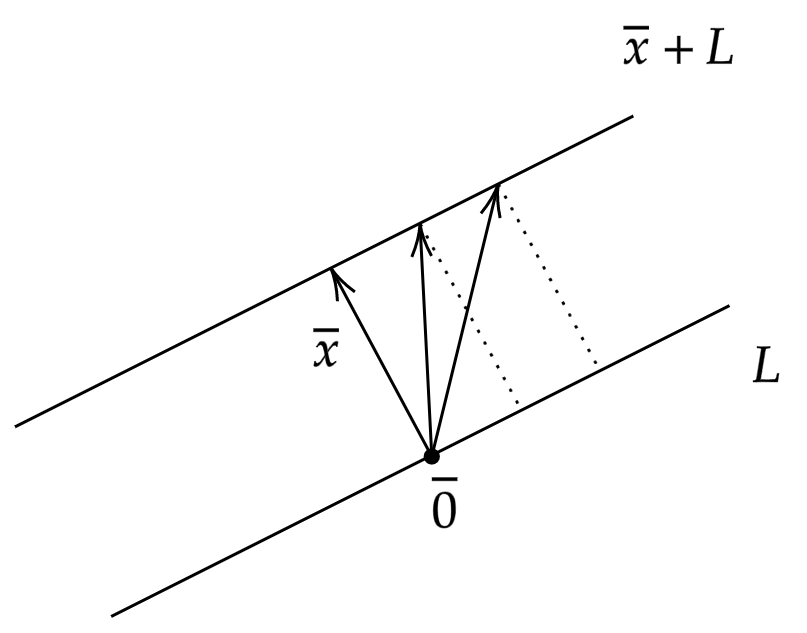
\includegraphics[width=6cm]{quotient_space}
    \caption{Ejemplo de espacio cociente}
    \label{quotient_space_picture}
\end{figure}

Como se ve en la figura, para identificar los \textit{subespacios paralelos}, debemos identificar todos los vectores tales que su resta (que es el vector que va desde un vector hasta el otro) pertenece al subespacio. Partiendo de esto, definimos la relación de equivalencia $\sim$ con la que trabajaremos el resto del texto.

\begin{definition}
    Sea $L \in \subespaciosde{V}$. En $V$ se define la relación binaria $\vx \sim \vy \iff \vx - \vy \in L$ 
\end{definition}

Veamos que efectivamente es de equivalencia.

\begin{proposition}
    $\sim$ es una relación de equivalencia. 
\end{proposition}

\begin{proof}
    Estudiamos las propiedades de la definición \ref{definicion_relacion_equivalencia} por separado.
    \begin{enumerate}[]
        \item Reflexividad. Como $L$ es un subespacio vectorial, entonces $\zv \in L$. Además, $\vx - \vx = \zv \in L$, por lo que $\vx \sim \vx$.
        \item Simetría. Sean $\vx, \vy \in V$. Veamos que $\vx \sim \vy \Rightarrow \vy \sim \vx$. Si $\vx \sim \vy$, entonces $\vx - \vy \in L$.
        \[
            \vy - \vx = \underbrace{\parens{-1}}_{\in \K}\cdot \underbrace{(\vx - \vy)}_{\in L} \in L
        \]
        Por tanto, $\vx \sim \vy \Rightarrow \vy \sim \vx$.
        \item Transitividad. Sean $\vx, \vy, \vz \in V \st \vx \sim \vy, \vy \sim \vz$. Demostremos que $\vx \sim \vz$.
        
        \[
        \begin{cases}
            \vx \sim \vy \\
            \vy \sim \vz 
        \end{cases} \Rightarrow \spc
        \begin{cases}
            \vx - \vy \in L \\
            \vy - \vz \in L
        \end{cases} \Rightarrow \spc
        \underbrace{\parens{\vx - \vy}}_{\in L} + \underbrace{\parens{\vy - \vz}}_{\in L} = \vx - \vz \in L 
        \]
        Por tanto, $\vx \sim \vz$
    \end{enumerate}
\end{proof}

Ahora que hemos demostrado que $\sim$ es una relación de equivalencia, podemos hablar de sus clases de equivalencia. Hallemos una caracterización que nos permita trabajar de manera cómoda con ellas. 

\begin{remark}
    Si $\vx \in V$, entonces
    \begin{align*}
        [\vx] &= \set{\vy \in V : \vy \sim \vx} = \set{\vy \in V : \vy - \vx \in L} = \set{\vy \in V : \exists \vec{l} \in L \st \vy = \vx + \vec{l}} \\
              &= \set{\vx + \vec{l} : \vec{l} \in L}
    \end{align*}
\end{remark}

Como vemos, la clase de equivalencia de un vector se consigue sumando a ese vector todos los vectores de $L$. Por ello, haremos el siguiente pequeño abuso de notación.

\begin{notation}
    Si $\vx \in V$, denotamos la clase de equivalencia de $\vx$ como $\vx + L = [\vx]$. 
\end{notation}

Nótese que no estamos sumando un vector con un subespacio, sino que únicamente es notación para la clase de equivalencia de $\vx$ bajo $\sim$.

Con las clases de equivalencia definidas, podemos definir el cociente.
\begin{definition}[Cociente]
    Llamaremos cociente de $V$ con $L$ a
    \[
        \faktor{V}{L} = \faktor{V}{\sim} = \set{[\vx] : \vx \in V} = \set{\vx + L : \vx \in V}
     \]
     Diremos que cocientamos $V$ con $L$.
\end{definition}

Normalmente utilizaremos la notación $\faktor{V}{L}$ para remarcar el subespacio vectorial $L$ con el que definimos la relación $\sim$.

Ahora que hemos definido el cociente, nos gustaría que fuese un espacio vectorial, para poder aplicar toda la teoría que estamos desarrollando. Definiremos operaciones sobre él (suma y producto por escalar) de manera que sean compatibles con las de $V$ y demostraremos que el cociente es efectivamente un espacio vectorial.

\begin{definition}[Suma en el cociente]
    \label{definicion_suma_cociente}
    En el cociente $\faktor{V}{L}$ definimos la operación suma como
    \begin{align*}
        + : \qs{V}{L} \times \qs{V}{L} & \to \qs{V}{L} \\
            \parens{\vx + L, \vy + L } & \mapsto \parens{\vx + \vy} + L
    \end{align*}
    Denotaremos entonces la suma como $\parens{\vx + L} + \parens{\vy + L} = \parens{\vx + \vy} + L$
\end{definition}

Como toda operación en cocientes, debemos demostrar que está bien definida.
\begin{proposition}
    La suma definida en $\qs{V}{L}$ en la definición \ref{definicion_suma_cociente} está bien definida.
\end{proposition}
\begin{proof}
    Sean $\vx', \vy' \in V$ tales que $\vx' \sim \vx$ y $\vy' \sim \vy$. Demostremos que $\parens{\vx + \vy} + L = \parens{\vx' + \vy'}+L$. Efectivamente,
    \[
        \begin{cases}
            \vx \sim \vx' \\
            \vy \sim \vy' 
        \end{cases} \Rightarrow \spc
        \begin{cases}
            \vx - \vx' \in L \\
            \vy - \vy' \in L
        \end{cases}
    \]

    Sumando ambos términos de la derecha tenemos que 
    \[
        \parens{\vx' + \vy'} - \parens{\vx + \vy} \in L \Rightarrow \parens{\vx'+\vy'} + L = \parens{\vx + \vy} + L
    \]
\end{proof}

Ahora que hemos demostrado que la suma está bien definida, para demostrar que $\qs{V}{L}$ es un espacio vectorial, debemos demostrar que cumple las propiedades relacionadas con la suma (demostraremos ahora las que únicamente están relacionadas con la suma, pues todavía no hemos definido producto por escalar) de la definición \ref{vector_space_definition} de espacio vectorial. 

Estas propiedades caracterizan una estructura algebraica muy útil, que se llama \textit{grupo abeliano}. Existen también los \textit{grupos} no necesariamente \textit{abelianos}. La única diferencia es que los grupos abelianos son conmutativos, mientras los grupos no deben por qué serlo.

\begin{definition}[Grupo abeliano]
    \label{definicion_grupo_abeliano}
    Un grupo abeliano es un conjunto $A$ con una operación  $+ : A \times A \to A$ que satisface las siguientes propiedades:
    \begin{enumerate}
        \item Conmutatividad. $\forall a, b \in A, \spc a + b = b + a$
        \item Asociatividad. $\forall a, b, c \in A, \spc \parens{a + b} + c = a + \parens{b+c}$
        \item Elemento neutro. Existe un elemento neutro $0 \in A$ tal que $0 + a = a + 0 = a \spc \forall a \in A $
        \item Elemento opuesto. $\forall a \in A, \spc \exists \parens{-a} \in A \st a + \parens{-a} = 0$.
    \end{enumerate}
\end{definition}

Demostraremos fácilmente gracias a la compatibilidad de la suma en el cociente con la suma en el espacio vectorial, que efectivamente se satisfacen estas propiedades.

\begin{proposition}
    \label{proposicion_cociente_grupo_abeliano}
    $\qs{V}{L}$ con la operación $+$ definida anteriormente es un grupo abeliano.
\end{proposition}

\begin{proof}
    Estudiemos una por una las propiedades de la definición \ref{definicion_grupo_abeliano}.

    \begin{enumerate}
        \item Conmutatividad. 
        \[
            \forall \vx, \vy \in V, \spc \parens{\vx + L} + \parens{\vy + L} = \parens{\vx + \vy} + L = \parens{\vy + \vx} + L = \parens{\vy + L} + \parens{\vx + L}    
        \] 
        \item Asociatividad.
        \begin{align*}
            \forall \vx, \vy, \vz &, \spc \parens{\parens{\vx + L} + \parens{\vy + L}} + \parens{\vz + L} = \parens{\parens{\vx + \vy} + L} + \parens{\vz + L} = \parens{\parens{\vx + \vy} + \vz} + L \\
            &= \parens{\vx + \parens{\vy + \vz}} + L = \parens{\vx + L} + \parens{\parens{\vy + L} + \parens{\vz + L}}
        \end{align*}
        \item Elemento neutro. Veamos que $\zv + L = \set{\vec{l} : \vec{l} \in L}$ es el elemento neutro. Sea $\vx \in V$,
        \[
            \parens{\vx + L} + \parens{\zv + L} = \parens{\vx + \zv} + L = \vx + L
        \]
        \item Elemento opuesto. Sea $\vx \in L$. Veamos que el opuesto de $\vx + L$ es $\parens{-\vx} + L$.
        \[
            \parens{\parens{-\vx} + L} + \parens{\vx + L} = \parens{-\vx + \vx} + L = \zv + L
        \]
    \end{enumerate}
\end{proof}

Definamos ahora el producto por un escalar. 
\begin{definition}[Producto por escalar en el cociente]
    \label{definicion_producto_escalar_cociente}
    En el cociente $\qs{V}{L}$ definimos el producto por un escalar como la aplicación
    \begin{align*}
        \cdot : \K \times \qs{V}{L} &\to \qs{V}{L} \\
                \parens{a, \vx + L}                    &\mapsto \parens{a \cdot \vx} + L
    \end{align*}
    Denotaremos el producto como $a \cdot \parens{\vx + L} = \parens{a \cdot \vx} + L$
\end{definition}

De nuevo, debemos demostrar que el producto está bien definido.

\begin{proposition}
    El producto por escalar definido en $\qs{V}{L}$ en la definición \ref{definicion_producto_escalar_cociente} está bien definido. 
\end{proposition}

\begin{proof}
    Sea $\vx'$ tal que $\vx \sim \vx' \Rightarrow \vx - \vx' \in L$. Por tanto, si $a \in \K$,
    \[
        a \cdot \vx - a \cdot \vx' = \underbrace{a}_{\in \K} \cdot \underbrace{\parens{\vx - \vx'}}_{\in L} \in L
    \]
    Por tanto, $a \vx \sim a \vx' \Rightarrow a \vx + L = a \vx' + L$
\end{proof}

Demostremos que con estas operaciones $\qs{V}{L}$ es un espacio vectorial.

\begin{proposition}
    El cociente $\qs{V}{L}$ con las operaciones definidas anteriormente es un espacio vectorial.    
\end{proposition}
\begin{proof}
    Analizemos por separado las propiedades de la definicion \ref{vector_space_definition}. Ya hemos demostrado que $\parens{\qs{V}{L}, +}$ es un grupo abeliano en la proposición \ref{proposicion_cociente_grupo_abeliano}, así que hemos demostrado las ppropiedades de la 1 a la 4. Veamos las restantes propiedades.
    \begin{enumerate}
        \setcounter{enumi}{4}
        \item Distributiva vectorial. Sea $a \in \K$ y $\vx, \vy \in V$. Entonces,
            \begin{align*}
                a \cdot \parens{\ecl{\vx} + \ecl{\vy}} &= a \cdot \ecl{\parens{\vx + \vy}} = \parens{a \cdot \parens{\vx + \vy}} + L = \parens{a\vx + a\vy} + L \\
                &= \ecl{a\vx} + \ecl{a\vy} = a \ecl{\vx} + a\ecl{\vy}
            \end{align*}
        \item Distributiva escalar. Sean $a, b \in \K$ y sea $\vx \in V$. 
        \begin{align*}
            \parens{a+b}\ecl{\vx} &= \parens{\parens{a+b}\vx} + L = \parens{a \vx + b \vx} + L = \ecl{\parens{a \vx}} + \ecl{\parens{b \vx}} \\
            &= a \ecl{\vx} + b \ecl{\vx}
        \end{align*}
        \item Asociativa. Sean $a, b \in \K$ y sea $\vx \in V$.
        \[
            \parens{a \cdot b} \ecl{\vx} = \parens{\parens{a \cdot b}\vx} + L = \parens{a \cdot \parens{b \cdot \vx}} + L = a \cdot \ecl{\parens{b \vx}} = a \cdot \parens{b \cdot \ecl{\vx}}
        \]
        \item Elemento unidad. Sea $\vx \in V$.
        \[
            1 \cdot \ecl{\vx} = \parens{1 \cdot \vx} + L = \vx + L
        \]
    \end{enumerate}
\end{proof}

Ahora que hemos demostrado que es un espacio vectorial, podemos hablar de su dimensión. Resulta que existe una expresión muy cómoda para la dimensión del cociente.

\begin{theorem}
    \label{dimension_cociente}
    \[
        \dim{\qs{V}{L}} = \dim{V} - \dim{L}
    \]
\end{theorem}

\begin{proof}
    Sea $\set{\vlst{u}{r}}$ una base de $L$ que vamos a extender a una base $\set{\vlst{u}{r}, \vu_{r+1}, \dots, \vu_n}$ de $V$. Veamos que $\mathcal{B} = \set{\vu_{r+1} + L, \vu_{r+2} + L, \dots, \vu_n + L}$ es base de $\qs{V}{L}$, con lo que quedaría demostrado el teorema, al ser $\dim{V} = n$ y $\dim{L} = r$.
    \begin{enumerate}
        \item Sistema de generadores. Veamos que $\mathcal{B}$ es sistema de generadores. Para todo $\vx \in V$ existen $\cslst{a}{n}{r} \in \K$ tales que
        \[
            \vx = \lincomb{a}{u}{r} + \underbrace{a^ {r+1} \vu_{r+1} + \dots + a^n \vu_n}_{\vy}
        \] 
        Con esa definición de $\vy$, si restamos $\vx - \vy$, al tener que $\set{\vlst{u}{r}}$ es base de $L$,
        \[
            \vx - \vy = \lincomb{a}{u}{r} \in L
        \]
        Por lo que,
        \begin{align*}
            \vx + L &= \vy + L = \parens{a^{r+1}\vu_{r+1} + a^{r+2}\vu{r+2} \dots + a^n \vu_n} + L \\
                    &= \ecl{\parens{a^{r+1}\vu_{r+1}}} + \ecl{\parens{a^{r+2}\vu_{r+2}}} + \dots + \ecl{\parens{a^{n}\vu_{n}}} \\
                    &= a^{r+1} \ecl{\vu_{r+1}} + a^{r+2} \ecl{\vu_{r+2}} + \dots + a^n \ecl{\vu_n}
        \end{align*}

        \item Linealmente independiente. Veamos que $\mathcal{B}$ es l.i. . Sean $a^{r+1}, a^{r+2}, \dots a^ n \in \K$ tales que 

        \[
            \underbrace{a^{r+1}\ecl{\vu_{r+1}} +  a^{r+2}\ecl{\vu_{r+2}} + \dots + a^{n}\ecl{\vu_{n}}}_{\parens{a^{r+1}\vu_{r+1} + a^{r+2}\vu_{r+2} + \dots + a^{n}\vu_{n}} + L} = \zv + L
        \]

        Por tanto,
        \[
            a^{r+1}\vu_{r+1} + a^{r+2}\vu_{r+2} + \dots + a^{n}\vu_{n} - \cancel{\zv} \in L
        \]

        Eso quiere decir que $\exists \slst{a}{r} \in \K$ tal que
        \[
            a^{r+1}\vu_{r+1} + a^{r+2}\vu_{r+2} + \dots + a^{n}\vu_{n} = \lincomb{a}{u}{r}
        \] 
        Pasando todos los términos a la izquierda restando llegamos a que,
        \[
            \parens{-a^1}\vu_1 + \parens{-a^2}\vu_2 + \dots + \parens{-a^r}\vu_r + a^{r+1}\vu_{r+1} + a^{r+2}\vu_{r+2} + \dots + a^{n}\vu_{n} = 0
        \]

        Como $\set{\vlst{u}{r}, \vu_{r+1}, \dots, \vu_n}$ es base de $V$, entonces en concreto son linealmente independientes, por lo que
        \[
            -a^1=-a^2= \dots = -a^r=a^{r+1} = a^{r+2} = \dots = a^n = 0
        \]
        Por tanto, $\mathcal{B}$ es linealmente independiente.
    \end{enumerate}
\end{proof}

\begin{remark}
    La demostración del teorema \ref{dimension_cociente} no solo nos dice la dimensión del cociente, sino que también nos proporciona una forma de encontrar una base de $\qs{V}{L}$. Para ello, tomamos una base de $L$ y la extendemos a una base de $V$. Los clases de los vectores añadidos forman una base del cociente.
\end{remark}

Veamos esto con más detalle en el siguiente ejemplo. Las ecuaciones de un subespacio y los determinantes se estudiarán con más detalle en siguientes secciones, aunque haremos uso de ellas para resolver este ejemplo.

\begin{example}
    Sea $L \subseteq \R^5$ el subespacio que tiene las ecuaciones canónicas 
    \[
        L \equiv \systeme{
            x_1 + x_2 + x_3 + x_4 + x_5 = 0, 
            x_2 - x_3 + x_5 = 0, 
            x_1 - x_2 + x_4 = 0,  
            x_1 - x_3 + x_4 + x_5 = 0
            }
    \]
    Determinar una base de $\qs{\R^5}{L}$ y, en dicha base, calcular las coordenadas de $\parens{0, 2, -3, 0, -1} + L$ en dicha base
\end{example}
\begin{solution}
Primero vamos a calcular una base de $L$ para extenderla a una de $V$. Nos damos cuenta de que la cuarta ecuación es la segunda más la tercera, por lo que podemos eliminarla resultando
\[
    L \equiv \systeme{
        x_1 + x_2 + x_3 + x_4 + x_5 = 0, 
        x_2 - x_3 + x_5 = 0, 
        x_1 - x_2 + x_4 = 0
        }
\]

Dejamos a la izquierda $x_1, x_2, x_3$ y pasamos a la derecha $x_4, x_5$
\[
    L \equiv \systeme{
        x_1 + x_2 + x_3 = - x_4 - x_5, 
        x_2 - x_3 = - x_5, 
        x_1 - x_2 = - x_4
        }
\]

Vemos que las ecuaciones son independientes porque 
\[
\det\mat{
    0 & 1 & 1 \\
    0 & 1 & -1 \\
    1 & -1 & 0 
} = -1 -1 -1 = -3 \ne 0
\]

Tenemos 3 ecuaciones independientes y $\dim{R^5}=5$, por lo que $\dim{L} = 2$. Esto lo veremos más adelante en el capítulo 3. Como $\dim{L}=2$, necesitamos dos vectores para la base. Si fijamos $x_4, x_5$, entonces tendremos un sistema de Cramer con solución única. Existen entonces dos vectores $\parens{a_1, a_2, a_3, 1, 0}, \parens{b_1, b_2, b_3, 0, 1} \in L$. A pesar de desconocer los valores $a_i, b_j$, sabemos que $\set{\parens{1, 0, 0, 0, 0}, \parens{0, 1, 0, 0, 0}, \parens{0, 0, 1, 0, 0}}$ completan la base porque desarrollando el determinante primero por las últimas columanas tenemos que
\[
  \det\mat{
      a_1 & b_1 & 1 & 0 & 0 \\
      a_2 & b_2 & 0 & 1 & 0 \\
      a_3 & b_3 & 0 & 0 & 1 \\
      1 & 0 & 0 & 0 & 0 \\
      0 & 1 & 0 & 0 & 0
  } \ne 0
\]

Aún así, si quisieramos calcular $a_i$ y $b_j$, que no nos es necesario para resolver el problema, solamente hace falta resolver el sistema asociado a fijar $x_4 = 1, x_5 = 0$ y $x_4 = 0, x_5 = 1$ en las ecuaciones de $L$. 

Por la demostración del teorema \ref{dimension_cociente} sabemos que una base del cociente son las clases de equivalencia de los vectores que completan la base de $L$, por lo que una posible base del cociente es
\[
    \mathcal{B} = \set{\parens{1, 0, 0, 0, 0} + L, \parens{0, 1, 0, 0, 0} + L, \parens{0, 0, 1, 0, 0} + L}
\]

Calculemos ahora las coordenadas de $\parens{0, 2, -3, 0, -1} + L$ en la base $\mathcal{B}$. Para ello, queremos hallar $\alpha, \beta, \gamma \in \K$ tal que
\begin{align*}
    \parens{0, 2, -3, 0, -1} + L &= \alpha \ecl{\parens{1, 0, 0, 0, 0}} + \beta \ecl{\parens{0, 1, 0, 0, 0}} + \gamma \ecl{\parens{0, 0, 1, 0, 0}} \\
                                 &= \parens{\alpha, \beta, \gamma, 0, 0} + L
\end{align*}

Como queremos entonces que las clases de equivalencia sean las mismas, esto es equivalente a que $\parens{\alpha, \beta, \gamma, 0, 0} \sim \parens{0, 2, -3, 0, -1}$, es decir, 
\[
    \parens{\alpha, \beta, \gamma, 0, 0} - \parens{0, 2, -3, 0, -1}  = \parens{\alpha, \beta-2, \gamma+3, 0, 1} \in L
\]
Para que ese vector pertenezca a $L$, debe verificar las ecuaciones del subespacio, es decir, $\alpha, \beta, \gamma$ deben verificar
\[
    \systeme{
        \alpha + \parens{\beta - 2} + \parens{\gamma} = -1, 
        \parens{\beta - 2} - \parens{\gamma + 3} = -1, 
        \alpha - \parens{\beta - 2} = 0
        } \iff \systeme*{
            \alpha = -\frac{2}{3},
            \beta = \frac{4}{3},
            \gamma = -\frac{8}{3}
        }
\]
Donde las coordenadas $\alpha,\beta,\gamma$ se han hallado resolviendo el sistema lineal de ecuaciones.
\end{solution}


\end{document}